\documentclass[12pt]{elsarticle}

%MATH
\usepackage{amsmath}
\usepackage{amssymb}
\usepackage{braket}

%TABLE
\usepackage{array}
\usepackage{multirow}

%GRAPHICS
\usepackage{graphicx}
\usepackage[caption=false,font=footnotesize]{subfig}
\graphicspath{{figures/}}
\DeclareGraphicsExtensions{.pdf,.jpg,.jpeg,.png}
\usepackage{tikz}
\usetikzlibrary{arrows.meta,shapes.geometric,calc,shadows}
\usepackage{forest}

%TYPEFACE
\usepackage{ulem}
\usepackage{soul}
\soulregister\cite7
\soulregister\ref7

%ENVIRONMENTS (GENERAL)
\usepackage{float}
\usepackage{standalone}
\usepackage{mdwlist}
\usepackage{hyperref}

%BIBLIOGRAPHY
\bibliographystyle{elsarticle-num}

\newif\ifappendix
\appendixtrue

\hyphenation{net-works MATLAB infra-structure MATPOWER DIgSILENT}

\journal{Reliability Engineering and System Safety}

\begin{document}
\begin{frontmatter}

%SSS - Title is clunky
\title{Identification of Interdependencies and Prediction of Fault Propagation for Cyber-Physical Systems}

\author[romeo]{Koosha~Marashi}
\ead{koosha@romeopower.com}
\author[s_and_t]{Sahra~Sedigh~Sarvestani\corref{cor}}
\ead{sedighs@mst.edu}
\author[s_and_t]{Ali~R.~Hurson}
\ead{hurson@mst.edu}

\address[romeo]{Romeo Power Technology, Vernon, CA 90058, USA}
\address[s_and_t]{Missouri University of Science and Technology, Rolla, MO 65409, USA}
\cortext[cor]{Corresponding author}

\begin{abstract}
\sout{Interdependence is an intrinsic feature of cyber-physical systems. Cyber and physical components are tightly integrated with each other, and hence, a trivial impairment in a part of the system may affect several components, leading to a sequence of failures that collapses the entire system. In this paper, we seek to identify the interdependencies among the components of a cyber-physical system using correlation metrics as well as a heuristic causation analysis method. We also demonstrate applicability of neural networks for prediction of imminent failures given the current system state. The proposed prediction tool can help system operators to perform timely preventive actions and mitigate the consequences of accidental failures and malicious attacks. As a case study, we have analyzed two smart grid test cases based on IEEE power bus systems, namely, IEEE--14 and IEEE--57.}
\vspace{1em}

\hl{Interdependence among components is a defining feature of cyber-physical systems. The tight coupling of cyber and physical components can enable a trivial impairment in one part of a system to affect components in other parts,  causing a sequence of failures that collapses the entire system. In this paper, we illuminate interdependencies among the components of a cyber-physical system using correlation metrics, and a heuristic causation analysis method, respectively. Understanding of these interdependencies enables prediction of imminent failures, given the current system state. We illustrate the use of neural networks to this end, and demonstrate the proposed approach with case studies on  smart grids based on the IEEE--14 and IEEE--57  power bus systems. Our work can be used to elucidate and quantify the effect of component interdependencies on system-level operation, and underpins analysis, prediction, and mitigation of failure for cyber-physical systems.}
\end{abstract}

\begin{keyword}
cyber-physical systems \sep
interdependency \sep
fault propagation \sep
correlation and causation \sep
failure prediction \sep
neural networks \sep
smart grid
\end{keyword}

\end{frontmatter}

\section{Introduction}\label{sec:intro}
%-----Prologue-----%
Complex systems exhibiting a tight coupling between physical processes and cyber infrastructures are known as cyber-physical systems (CPSs). Computational capabilities and communication technologies have enabled development of CPSs that can achieve higher dependability standards and provide a better performance. The cyber infrastructure is the backbone of a CPS and provides wide-area measurement and monitoring, distributed control, and decision support.

%-----Background-----%
The tight coupling of the physical and cyber networks are through links and various means of interactions, which makes them intertwined systems with intense interdependencies. \emph{Interdependence} is a general term that accounts for a relationship among components of a system, where state of each component influences or is correlated with the state of others~\cite{RiP01}. Interdependence can be categorized into different types and may exist at different levels, i.e., between systems, subsystems, or components. For example, a malfunctioning fuel pressure sensor in a car affecting its fuel economy manifests a functional interdependency in the engine subsystem. In an interdependent CPS, impairments originating in cyber and physical components may propagate through unprotected channels and escalate into a system-level failure. In general, interdependencies in a system can severely complicate the development of accurate models. This paper seeks to present a model of interdependency for CPSs, and develop a tool for predicting the components that are in risk of failure by reason of an earlier impairment.

%-----Motivation-----%
There are numerous examples of large-scale systems being affected by impaired components or due to impairments in other correlated systems. The Arizona-Southern California blackout in September 2011, which occurred as a result of an 11-minute outage of a 500 kV transmission line is an example of cascading failures with profound consequences due to internal interdependencies within the boundaries of the Southwestern US power grid. The outage triggered a cascade that left approximately 2.7 million customers without power for up to 12 hours~\cite{FERC12}. The Italy blackout, occurred in September 2003, is another example in which interdependencies among different infrastructures caused further outages~\cite{BeA04}. This failure was exacerbated by the loss of Internet communication nodes left without power, which in turn caused further breakdown of communication and control at multiple power stations. Such incidents motivate our work on identification of cyber-physical interdependencies and prediction of imminent failures across the physical and cyber domains.

%-----Why is this work needed?-----%
The need for proper preparation and planning has been emphasized in the task force reports of aforementioned and several other catastrophic events~\cite{FERC12,BeA04,A14Rp}. An interdependency model is the key in providing the knowledge needed for preparedness. In a disruption cycle of a system, interdependency models can substantially help at three stages:
\begin{basedescript}{\desclabelstyle{\pushlabel}}
  \item[Before disruption:] Models can be developed to conduct simulations to improve awareness and understanding of the potential risks and their consequences, compare alternative recovery strategies, and enable contingency planning.
  \item[During disruption:] Availability of knowledge and resources aid decision--making to mitigate consequences and support rapid recovery.
  \item[After disruption:] Models can help in determining high-priority actions required for restoration of essential services as well as resources needed for supporting recovery. Models should be continually refined based on what was learned from the event.
\end{basedescript}

%-----Related Work-----%
Literature is abundant on the analysis of interdependency and its effects. In the area of critical infrastructure, Rinaldi et al. have provided an ontology for understanding interdependence and its classification into physical, cyber, geographic, and logical~\cite{RiP01}.
%-----RW: Identification-----%
Researchers have used different approaches to identify interdependence among components, systems, or operations. In~\cite{LaK07}, the interdependencies between electrical infrastructure and the associated information infrastructure are qualitatively investigated and the pattern of fault propagation is explored. There are also examples of using correlation metrics for studying the interdependence. In~\cite{MeW06}, Pearson's correlation metric is used to investigate dependence among critical infrastructures after the World Trade Center attack. In another study~\cite{DuK12}, the time-series analysis method is utilized to reveal interdependencies across critical infrastructures from post-event restoration curves of February 2010 Chile earthquake. %The cross-correlations from the curves without significant lag times reflected the operational interdependencies, and those with significant lag times measured the logistical interdependencies.

%-----RW: Modeling-----%
Models of interdependency are presented using a variety of techniques such as topology-based and flow-based methods, Bayesian networks, and Petri nets. In~\cite{BeC12}, Beccuti et al. proposed an approach using stochastic Petri nets for modeling the operation of the physical and cyber networks in electric power delivery systems. They subsequently measured the effect of disruptions of one network on the other (e.g., as a result of a cyber attack) in terms of a number of domain-specific performance indices. \hl{The study presented in~\cite{ZhH18} utilizes graph-theoretic metrics to model cascading failures in power grids.  Topological constraints are applied to capture the impact of  load dynamics (physical domain) and node dependencies (cyber domain).   In~\cite{GuY19}, a Markovian process model is used to encapsulate both stochastic and deterministic behaviors of a failure propagation scenario in power systems. Although the cyber infrastructure is taken into account, the focus of the authors is mainly on  application of multi-agent control techniques to modern smart grids and investigating the effect of these techniques on cascading failures. Another recent study, presented in ~\cite{TuX19}, attempts to improve interdependency models by accounting for the resilience of a given cyber or physical component against failure of its counterpart in the other network. This resilience is modeled using two-way probabilistic internetwork dependency joints.}

%-----RW: Quantification-----%
Another group of studies are devoted to quantification of interdependencies. Casalicchio and Galli have presented a number of quantitative metrics for interdependencies in critical infrastructures and classified them into shape, core, and sector-specific metrics~\cite{CaG08}. Studies presented in~\cite{HuW15a,ZhG13} use topological metrics (e.g., connectivity and size of giant component) to quantify interdependency in a network; however, for the case of power grids, Verma et al. argue that topological measures that are not context-aware may underestimate vulnerability of the system~\cite{VeE15}.

%-----RW: Prediction-----%
As mentioned earlier, an important result of interdependency analysis is to predict the risk of failures for components and systems, prioritize preventive maintenance, and perform timely actions to mitigate effects of disruptions. In~\cite{GrB06}, statistical machine learning techniques were used to predict failure of feeder lines in boroughs of New York City over a three-month period and showed an acceptable accuracy of 75\%. Additional results on application of the proposed methods are presented in~\cite{RuW12}. \hl{ In~\cite{StS20}, graph theoretical methods are used to represent a power grid coupled with a communication network.  Supervised machine learning techniques, including polynomial and decision tree regression models, are trained with synthetic failure data to model the propagation of failures in the resulting cyber-physical power system.}

%-----Objectives and Contributions-----%
\sout{In this paper, our objective is to present a model of interdependency by observing sequence of failures for a set of failure cases and capturing the extent of interdependence with quantitative metrics as well as to provide a tool for prediction of failure sequences. We identify interdependencies among components of a CPS using correlation and causation analyses and quantify them with dependency metrics presented in our previous work ~\cite{MaS16}. Using the knowledge of the interdependency, we identify areas of the system where faults can propagate and create larger failures. We then create a set of failure cases and use the data from the resulting failure sequences to develop and configure an artificial neural network for prediction of fault propagation paths and cascading failures. Our research paves the road to a better understanding of interdependencies in a system and prediction of its future failures using historical failure records or data from simulation of failure scenarios. To illustrate our approach, we have applied it to two smart power grids based on the well-studied IEEE 14-bus and 57-bus test systems.}

\hl{Our proposed approach to analyzing interdependency begins with identification of likely failure cases for the system. Each system-level failure case describes a set of distinct components whose concurrent failure can cause a disruption to operation of the system. Dependency links carry the initial disruption to other components, causing them to fail. Observation of these secondary (and tertiary, and so on) failures is our means of inferring the underlying  dependencies among the components. We propose metrics for quantifying the extent of interdependence, and a model that predicts the sequence of failures triggered by a given disruption.

%SSS - unclear how we complement [18]
In this paper, we illustrate the use of correlation and causation analysis for identifying interdependencies among components of a cyber-physical system. We quantify the extent of interdependency with metrics proposed in our previous work~\cite{MaS16}. Using  knowledge of  interdependency, we identify areas of the system where faults can have an outsized effect, propagating and eventually causing consequential failures. We then create a set of failure cases and observe the sequence of failures triggered by each. The insights gained enable prediction of  fault propagation paths and cascading failures for the system. We illustrate the creation and configuration of an artificial neural network that brings these  predictive abilities to bear.  Through two case studies on smart grids based on  the well-studied IEEE 14-bus and 57-bus test systems, we demonstrate that a domain-specific cyber-physical simulation environment can capture the sensing, decision making, and control roles of discrete-time cyber components by reflecting their operation at the fine granularity required. In this respect, our proposed approach complements the work of Sturaro et al. in ~\cite{StS20}. Our work can be used to elucidate and quantify the effect of component interdependencies on system-level operation, and underpins analysis, prediction, and mitigation of failure for cyber-physical systems.}

\section{Interdependency Analysis}
\label{sec:analysis}
\emph{Dependency} is a linkage between two entities, through which the state of one entity influences or is correlated with the state of the other. In this case, the relationship is usually unidirectional, i.e., entity $i$ depends on $j$, but $j$ does not depend on $i$. The influence of one entity on another can be exerted through intermediate entities, and need not be direct. In this paper, our focus is on functional dependencies between components of a single CPS. As an example, correct operation of a software that determines control commands for actuators in a robotic system is contingent on correct data from a sensor that detects surrounding objects. In this case, the software depends on the sensor, but the sensor does not depend on the software, as it can continue its operation regardless of the state of the software.

% NJ - Why the focus on just interdependency?
The terms ``dependency'' and ``interdependency'' are often used interchangeably. In this paper, our usage will be precise. We consider \emph{interdependency} to describe \emph{bidirectional} dependency, i.e., the state of an entity influences or is correlated with the state of another, and vice versa. In other words, entity $i$ depends on $j$ through a number of links, and $j$ likewise depends on $i$, possibly through different links. The interconnected topology and tight functional coupling typical of CPSs creates significant interdependency among components.

\subsection{Representation of Interdependencies}
\label{sec:analysis:repr}
For representation of interdependencies in a CPS, we use \emph{dependency graph} that is a two-level weighted directed graph in which an edge exists from node $i$ to node $j$ if and only if the state of component $i$ impacts, in one time step, the state of component $j$. Given a time step of sufficiently short duration, we can assume that impairment of a component propagates to the others through direct links only, not through multiple intermediate links.

Depending on the source and destination of an edge, it can represent one of four types of dependency, namely, physical-physical, physical-cyber, cyber-physical, and cyber-cyber. Note that in this notation, $s_1-s_2$ represents a relation in which components of subsystem 1 ($s_1$) influence components of subsystem 2 ($s_2$). \figurename~\ref{fig:sample_dep_graph} illustrates a dependency graph for a hypothetical CPS and specifies these four types of dependency. Note that in this context, ``physical-cyber'' and ``cyber-physical'' represent different types of dependencies. For example in the 2003 Italy blackout~\cite{BeA04}, the loss of telecommunication services that occurred following the initial power outage manifests a physical-cyber dependency, while the additional outages in the grid that took place because of the loss of control in the power stations indicates a cyber-physical dependency.

In \figurename~\ref{fig:sample_dep_graph}, the bottom plane encompasses components of the physical system and the top plane is representative of the cyber infrastructure that monitors and controls the underlying physical processes. The weights shown on the edges represent the extent of dependency, denoted as the \emph{degree of influence} and are in the range of $[0, 1]$, where a 0 means that there is no functional influence from a component on another, and a 1 is the case where the state of a component causes maximal degradation to the state of another, i.e., makes it unable to operate.
% NJ - This is not strictly accurate -- we can have functional influence where when one power line fails, the load on the other doubles, but does not cause failure

\begin{figure}
\centering
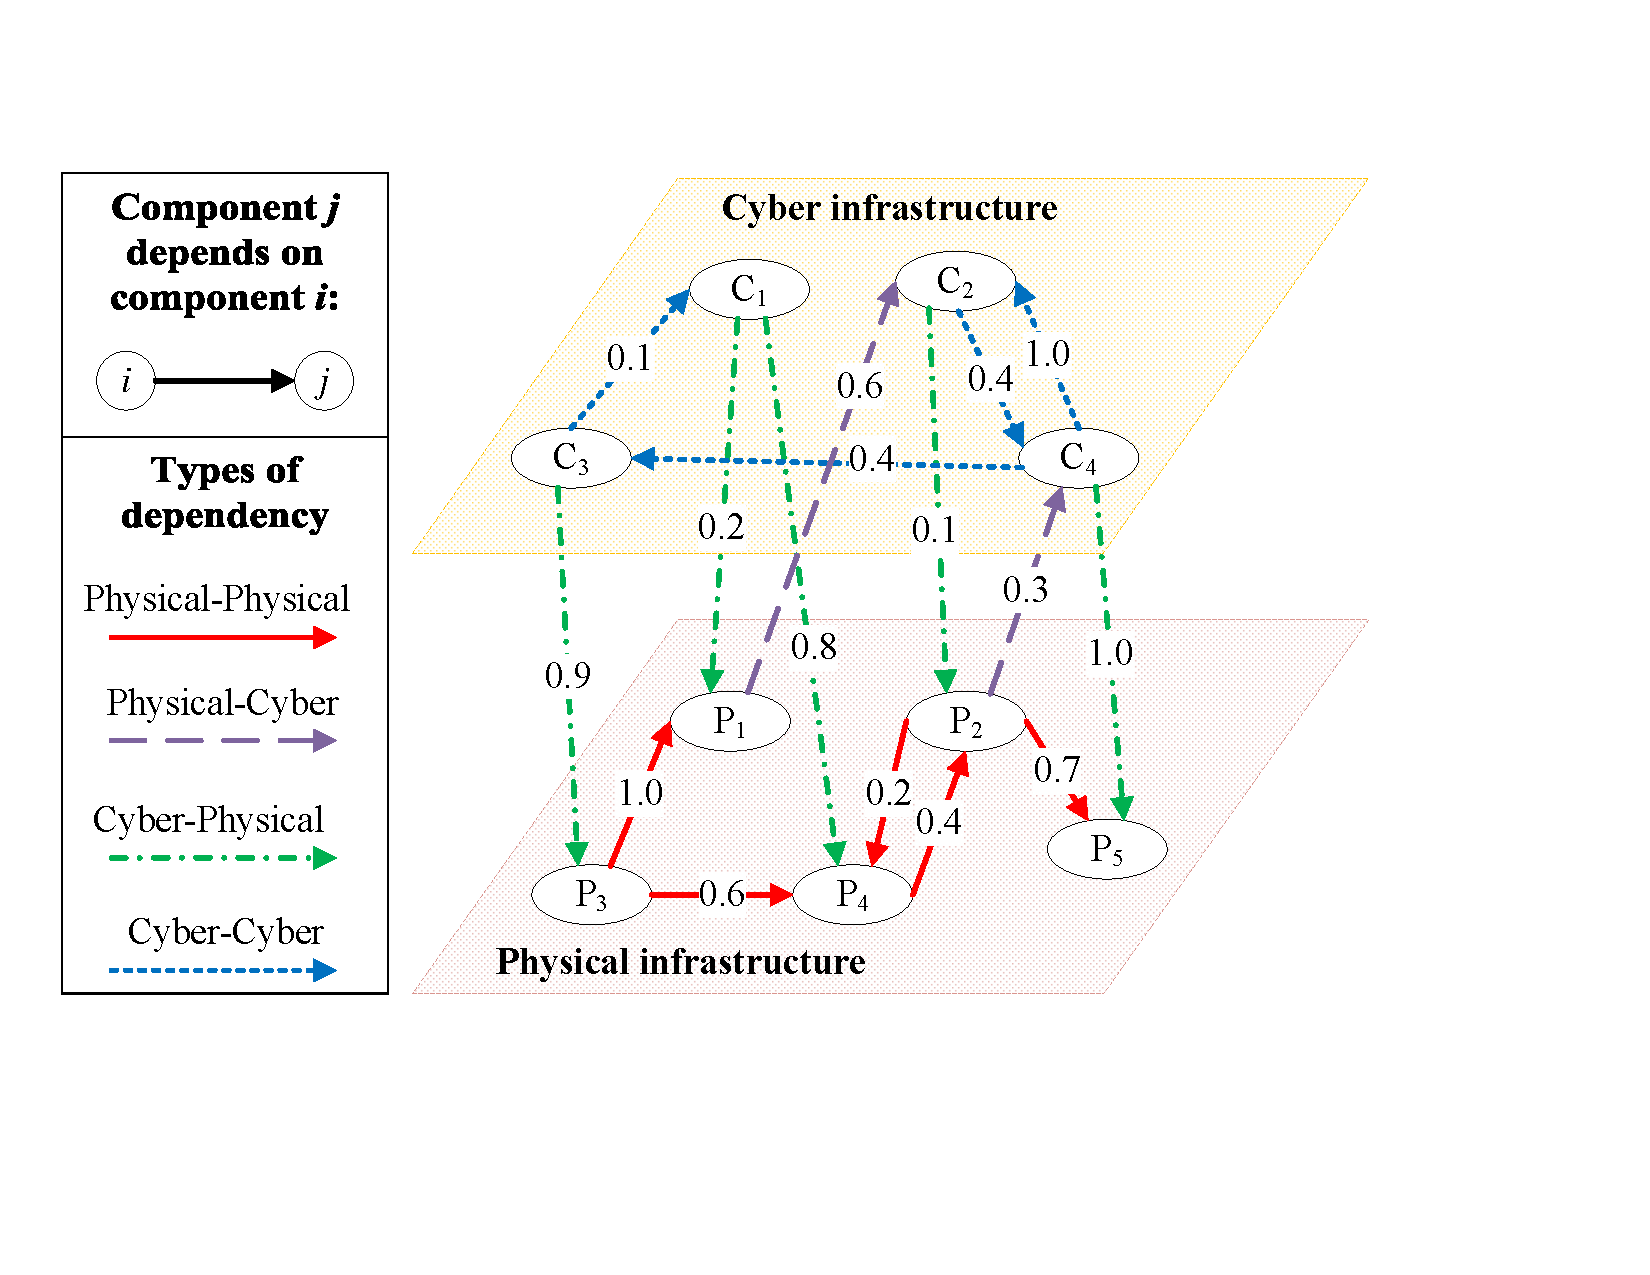
\includegraphics[width=0.70\columnwidth]{sample_dep_graph}
\caption{Dependency graph of a hypothetical CPS.}
\label{fig:sample_dep_graph}
\end{figure}

% NJ - Need to introduce $n$ here -- # of components
For mathematical representation, we introduce a \emph{direct influence matrix}, denoted as $\mathbf{D} = \left[d_{ij}\right] \in [0, 1]^{n \times n}$, which is in fact the adjacency matrix of the dependency graph. $d_{ij}$ represents the \emph{degree of influence} that component $i$ exerts on component $j$ and $n$ is the total number of components in the system. Note that the entries on the diagonal of $\mathbf{D}$ should always equal zero, as a faulty state of a component ``propagates'' to itself immediately, not after one time step.

\subsection{Identification of Interdependencies}
\label{sec:analysis:iden}
Interdependency between components can be due to causality or simply correlation. In a causation relationship, the state of a component is responsible for that of another. On the other hand, the state of two components are correlated when they have a statistical relationship, whether causal or not. In a simple system with a processor that controls two actuators, it may be observed that the two actuators fail together, however, no cause-and-effect relationship is established. In fact, further analysis may reveal that the failure of the processor unit causes failure of both actuators, hence indicates simultaneity (a type of correlation) between failure of the two actuators without one being the actual reason for failure of the other. Depending on the purpose of interdependency analysis, either correlation or causation may be of interest. In this section, we present two approaches for analysis of causation and correlation, respectively, by observing sequence of failures for a set of failure cases.

A \emph{failure case} describes a set of distinct components whose failure (assumed to be concurrent) initiates disturbance to the system. These initial disruptions, applied to the system at time $t=0$, may propagate to other components through dependency links. For the disturbance initiated by failure case $k$, let $\mathcal{F}_{k}(t)$ represent the set of components that are observed to be in a degraded state at time instant $t$. For failure case $k$, a \emph{failure sequence} of length $L$ represents $L$ consecutive observations of the system state and is denoted as $\mathcal{F}_{k}(t), 0 \leq t < L$.

Our approach to identification of dependencies relies on observation of the system's behavior in response to each of a set of failure cases. The disruption associated with each failure case triggers a failure sequence, from which we infer dependency links between the components. The extent of dependency can be quantified with statistical methods such as correlation or causation analysis. The greater the number of failure cases, and the longer the duration of observation for each, the more accurate this inference will be. For collecting the failure sequences, it is possible to utilize data from simulation, laboratory and/or field observation, and/or historical data about failures of a system. In this paper, we present our results using data from a simulation environment.

\subsubsection{Correlation Analysis}
\label{sec:analysis:iden:corr}

Correlation of two random variables reflects a statistical relationship, i.e., dependence between their values. A variety of existing measures can be used to quantify this dependence. For example, the Pearson correlation coefficient can capture linear dependence between two random variables. More sophisticated correlation measures can identify non-linear relationships as well and thus serve as powerful statistical tools for quantifying functional dependency between components.

For each component, we define a \emph{state variable}, which is a random variable that characterizes the state of the component, then determine correlation between these random variables. Let $X_i(t)$ denote the state variable of component $i$ at time $t$. For analysis of dependency of component $j$ on component $i$, Pearson correlation coefficient (PCC) between $X_i(t)$ and $X_j(t)$ is calculated, as shown in Equation~\eqref{eqn:pearson}.

\begin{equation}
\label{eqn:pearson}
\rho_{X_i X_j} = \dfrac{\text{cov}(X_i, X_j)}{\sigma_{X_i} \sigma_{X_j}}
\end{equation}

Where $\text{cov}(.)$ is the covariance and $\sigma$ is the standard deviation of a state variable. As noted in Section \ref{sec:analysis:repr}, we are interested in finding $d_{ij}$ values, which represent dependence in one time step. Furthermore, direction of relationship (increasing or decreasing) is not of our interest. Therefore, we use $PCC_{X_i X_j} = |\rho_{X_i(t) X_j(t + 1)}|$ to capture the direct dependency.

A shortcoming of PCC is that it only detects linear relationships, while an impaired component may result in disturbances in another component that are not necessarily linear. From various correlation coefficients introduced for detecting nonlinear relationships, we selected \emph{randomized dependence coefficient} (RDC)~\cite{LoH13}, which has a low computational complexity and shows a good performance in comparison with similar methods. Readers are referred to~\cite{LoH13} for more information on RDC. In this paper, we use $RDC_{X_i X_j}$ notation to represent RDC correlation between state variables $X_i$ and $X_j$. Note that RDC has two parameters associated with it: sample size and number of random features, which are set following guidelines provided in~\cite{LoH13}.

For identification of interdependencies we can compute the mean value of correlation coefficients (either PCC or RDC) between $X_i$ and $X_j$ over all failure cases and use it as an estimator for $d_{ij}$.%, as shown in Equation~\eqref{}.

%\begin{eqnarray}
%\label{eqn:d_pcc}
%\hat{\mathbf{D}}_{PCC} &=& \left[\hat{d}_{PCC, ij}\right], \quad \hat{d}_{PCC, ij} = \sum\limits_ \\
%\label{eqn:d_rdc}
% &=& 
%\end{eqnarray}

\subsubsection{Causation Analysis}
\label{sec:analysis:iden:caus}
In general, a causal relationship is harder to establish than correlation, and hence, fewer interdependency studies have investigated causality. We use a method inspired by the interaction model introduced in~\cite{QiS15} to identify causation relationships and estimate $\mathbf{D}$. The work presented in~\cite{QiS15} determines the interactions among components of a power grid, finds key dependency links, and provides strategies for mitigating cascading failures using a heuristic method. We present a similar method that is generalized to be applicable for cyber-physical systems. Specifically, we have extended the method to incorporate heterogeneous components, control the sensitivity in detecting causality, and account for dependency relationships between degraded states rather than binary states. We utilize a cyber-physical simulation environment and account for discrete-time behaviors of the cyber infrastructure, which is not possible in the OPA simulation environment employed in~\cite{QiS15}. For validation of the basic proposed approach readers are referred to the original study~\cite{QiS15}.

% NJ - Need to clearly define w_{ij}
% NJ - Since W is used in H(t), should it be W(t) instead?
% NJ - Need to motivate the definition of H(t) and E
% NJ - Does W need to be normalized? This is perhaps not clear; I have a note that says 'see ref. 17' but no elaboration...
Consider a system composed of $n$ components, for which $m$ failure cases are observed. Recall that for a given failure case $k$, the set $\mathcal{F}_{k}(t)$ is composed of all components that experienced degradation at time $t$. From the set of all failure sequences, i.e., $\mathcal{F}_{k}(t), \forall k$, we can construct the failure succession frequency matrix, $\mathbf{W} = \left[w_{ij}\right] \in \mathbb{Z}^{n \times n}$, where $w_{ij}$ shows the number of times component $j$ has degraded one time step after degradation of component $i$ over all failure cases. Components in the set $\mathcal{F}_{k}(t - 1)$ whose states are known to be the dominant causes for degradation of component $j$ in $\mathcal{F}_{k}(t)$ are identified using Equation~\eqref{eqn:dominant_components}.

\begin{equation}
\label{eqn:dominant_components}
\mathcal{H}_{k, j}(t) = \set{i | i \in \mathcal{F}_{k}(t - 1), w_{ij} \geq \alpha \max\limits_{l \in \mathcal{F}_{k}(t - 1)} w_{lj}}
\end{equation}

In Equation \eqref{eqn:dominant_components}, $\alpha$ controls the threshold in detecting the causative relationships. Selection of $\alpha$ depends on the distribution of $w_{ij}$ among the members of $\mathcal{F}_{k}$ set. In the histogram shown in \figurename~\ref{wij_hist}, we observe a significant separation between the members of $\mathcal{F}_{k}$ at about $w_{ij} = 0.9$, which allows us to easily distinguish correlative and causative relationships. For the systems studied in this work, the $w_{ij}$ histograms follow a similar pattern to what is shown in \figurename~\ref{wij_hist}. Therefore, in all following analyses, we set $\alpha$ to 0.9 (shown as a red dotted line on \figurename~\ref{wij_hist}), i.e., $\mathcal{H}_{k, j}$ captures members of $\mathcal{F}_{k}$ whose $w_{ij}$ value is larger than 0.9 (on the right of the red dotted line).

\begin{figure}
\centering
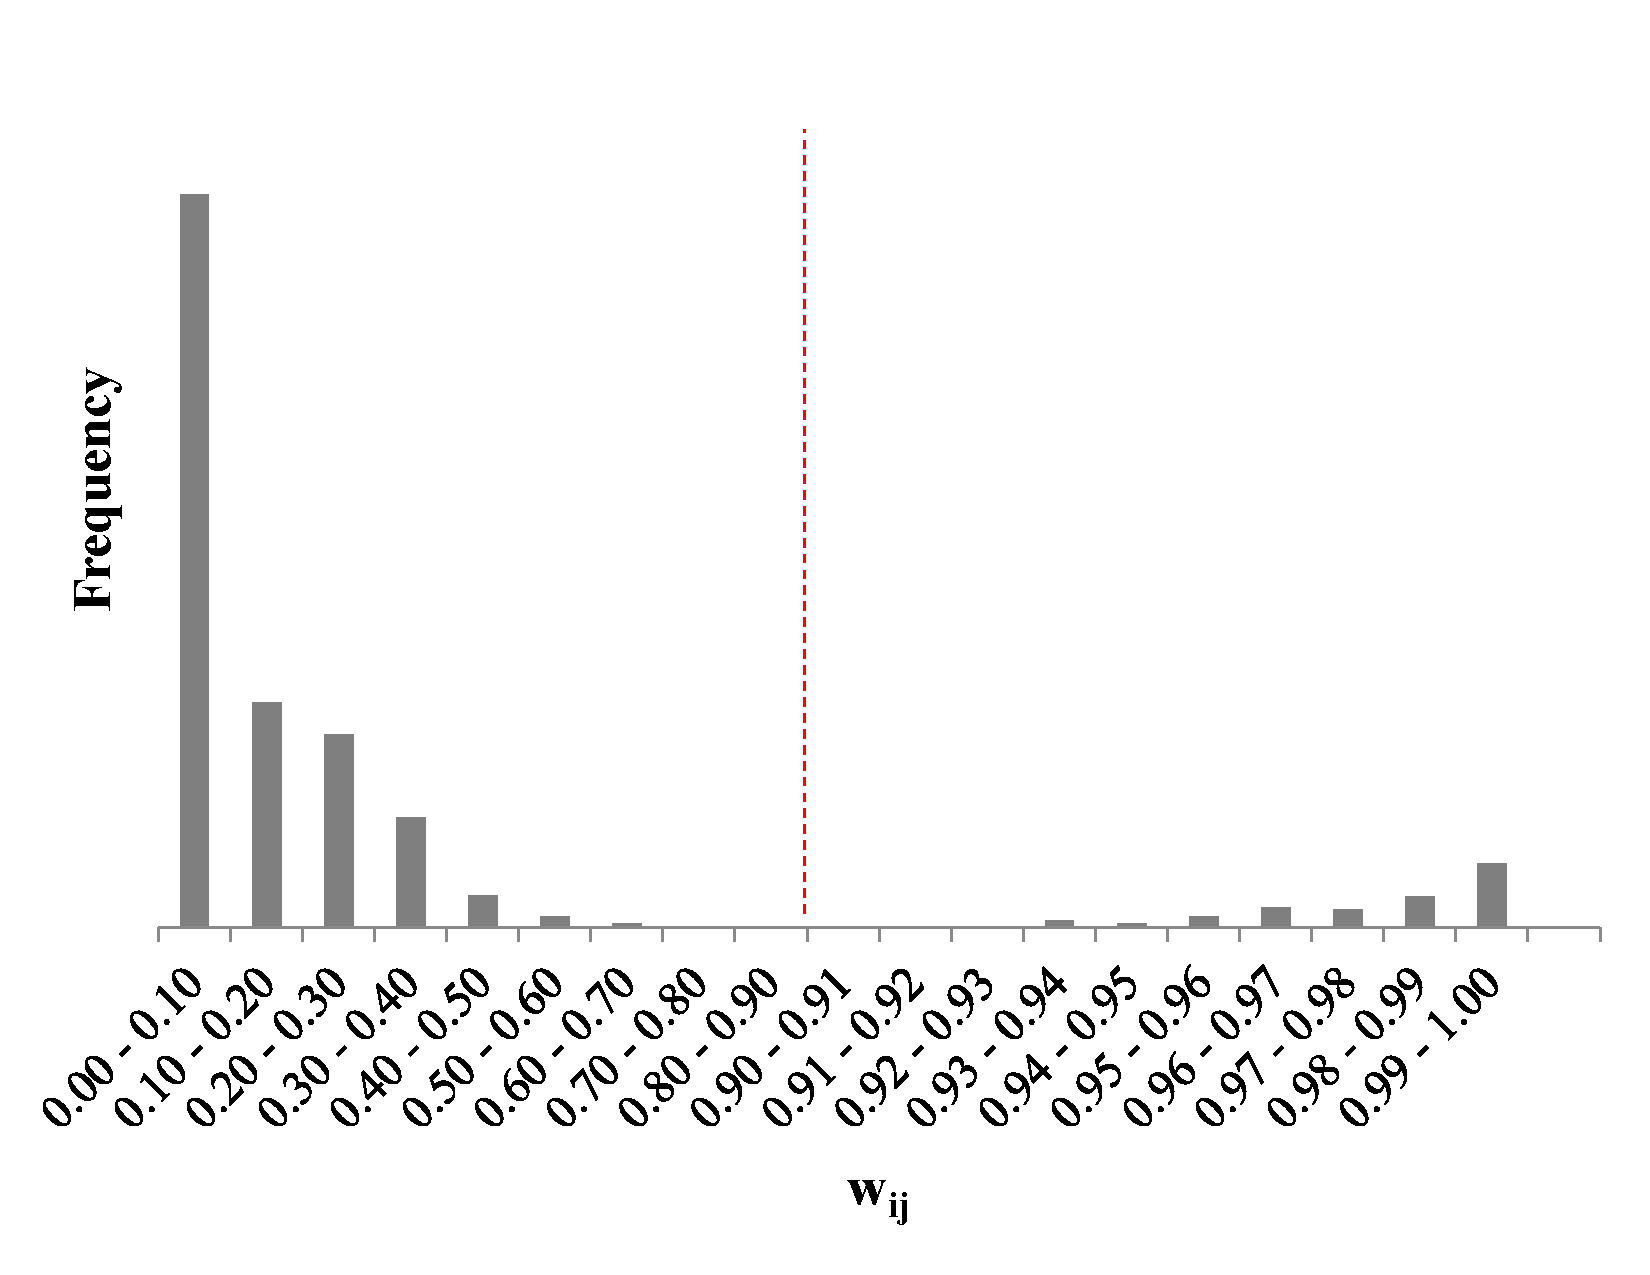
\includegraphics[width=0.7\columnwidth]{wij_hist}
\caption{Histogram of $w_{ij}$ among members of $\mathcal{F}_{k}$ in a representative system.}
\label{wij_hist}
\end{figure}

Matrix $\mathbf{E} = \left[e_{ij}\right] \in \mathbb{Z}^{n \times n}$ is constructed as shown in Equation~\eqref{eqn:matrix_e}, where $e_{ij}$ is the number of times degradation of component $i$ caused degradation of component $j$.

\begin{eqnarray}
\label{eqn:matrix_e}
\mathbf{E} &=& \left[e_{ij}\right] \nonumber \\
e_{ij} &=& \sum\limits_{k=1}^{m} \sum\limits_{t > 0} \text{card}({\set{(k, t) |i \in \mathcal{H}_{k, j}(t)}})
\end{eqnarray}

In Equation \eqref{eqn:matrix_e}, $\text{card}(.)$ denotes the cardinality of a set. Assuming that $N_i$ is the total number of times component $i$ experiences degradation over all failure cases, $\dfrac{e_{ij}}{N_i}$ estimates the likelihood of component $i$ having a causative relationship with component $j$. In other words, $\dfrac{e_{ij}}{N_i}$ represents the degree to which degradation of component $i$ ``causes'' degradation in component $j$.

\subsection{Quantification of Interdependencies}
\label{sec:analysis:quan}
Assuming that the direct influence matrix $\mathbf{D}$ is known, we can explore dependency of components in multiple time steps. Specifically, we are interested in the \emph{$k$\textsuperscript{th}-level influence matrix}, which represents the influence that components have on each other over exactly $k$ time steps -- in contrast to $\mathbf{D}$, where the influence exerted over a single time step is captured. To this end, we first normalize $\mathbf{D}$ by dividing it by $n$ to ensure that $\sum\limits_{j=1}^n d_{ij} \leq 1$. Matrix $\left(\frac{1}{n}\mathbf{D}\right)^k$ is hence guaranteed to have an upper bound, and represents the $k$\textsuperscript{th}-level influence matrix. The \emph{total influence matrix}, $\mathbf{T}$, can be computed as shown in Equation~\eqref{eqn:total_influence_matrix}.

\begin{eqnarray}
\label{eqn:total_influence_matrix}
\mathbf{T} &=& \left[t_{ij}\right] = \mathbf{V} \circ \sum\limits_{k = 1}^{\infty} \left(\frac{1}{n}\mathbf{D}\right)^k \nonumber \\
\mathbf{V} &=& [v_{ij}] \nonumber \\
v_{ij} &=&
\left\{
\begin{array}{ll}
  \dfrac{n+1}{n}, & \enskip i \neq j; \\[1em]
  \dfrac{n+1}{n-1}, & \enskip i = j.
\end{array}
\right.
, \enskip 1 \leq i,j \leq n
\end{eqnarray}

In Equation~\eqref{eqn:total_influence_matrix}, $\circ$ represents the entrywise product and  $t_{ij}$ shows the degree by which component $j$ can be influenced by a failure in component $i$ in any number of time steps, which reveals indirect influences. Note that the matrix $\mathbf{V}$ is used to scale $t_{ij}$ to $[0, 1]$ range.

In Equations \eqref{eqn:tau} and \eqref{eqn:nu}, we define $\tau_i$, and $\nu_j$, which are respectively the weighted out-degree of node $i$ and weighted in-degree of node $j$, in order to evaluate the extent of influence components exert on or receive from other components.

\begin{eqnarray}
\label{eqn:tau}
\tau_{i} &=& \frac{1}{n} \sum\limits_{j=1}^{n} t_{ij} \\
\label{eqn:nu}
\nu_{j} &=& \frac{1}{n} \sum\limits_{i=1}^{n} t_{ij}
\end{eqnarray}

We will also measure the average dependence that components of subsystem $s_1$ have on components of subsystem $s_2$. For this purpose, $\gamma_{s_1-s_2}$ is calculated as shown in Equation~\eqref{eqn:gamma_s}.

\begin{equation}
\label{eqn:gamma_s}
\gamma_{s_1-s_2} = \frac{1}{n_{s_1}n_{s_2}}\sum\limits_{i \in s_1} \sum\limits_{j \in s_2} t_{ij}
\end{equation}

In Equation~\eqref{eqn:gamma_s}, $n_{s_1}$ and $n_{s_2}$ are the number of elements in subsystems $s_1$ and $s_2$, respectively, and $n_{s_1} + n_{s_2} = n$. Note that $\tau$, $\nu$, and $\gamma_{s_1-s_2}$ are all normalized to the $[0, 1]$ range so that systems of different sizes can be easily compared.

\section{Prediction of Failure Sequences}
\label{sec:pred}
Upon availability of knowledge of interdependency among the components of a system, a prediction tool may be used to detect catastrophic failures in their incipient stage and enable the supervisory control team to perform timely preventive actions and make appropriate decisions to mitigate the consequences~\cite{AfM17,AfM18}. For this purpose, powerful and reliable tools are needed that are capable of identifying the components (or sections of the system) that are prone to failure as a result of a disruptive event. Furthermore, such tools are expected to respond in real-time and provide a prioritization of the components that are in risk, based on their failure likelihood and importance of their roles in the system.

The problem of predicting a sequence of events is closely related to classification and sequence labeling in time series analysis. In this work, we transform the problem of sequence prediction into a multi-class classification and investigate the use of artificial neural networks (ANN) for tackling this problem. Reports show that ANNs are a promising tool for classification problems~\cite{OuM07}. In a multi-class classification problem, a given instance is to be associated with a number of classes. The classification can also be probabilistic, where the classifier provides a probability distribution of a given instance belonging to the existing classes. Some of the popular classification problems are speech recognition, pattern recognition, and medical imaging.

For a system with $n$ components, let $\mathbf{X}(t) = \left(X_1(t), X_2(t), \ldots, X_n(t)\right)$ denote the input array to the ANN, where $X_i(t)$ is the state variable of component $i$ at the time instance $t$. $\mathbf{X}(t)$ is fed to a multi-layer fully connected ANN with the architecture shown in \figurename~\ref{nn_architecture}. The Output layer provides $\mathbf{Y} = \left(Y_1, Y_2, \ldots, Y_n\right)$, where $Y_i$ represents the probability that component $i$ fails as a result of the disruption specified by the given state variables in the input.

\begin{figure}
\centering
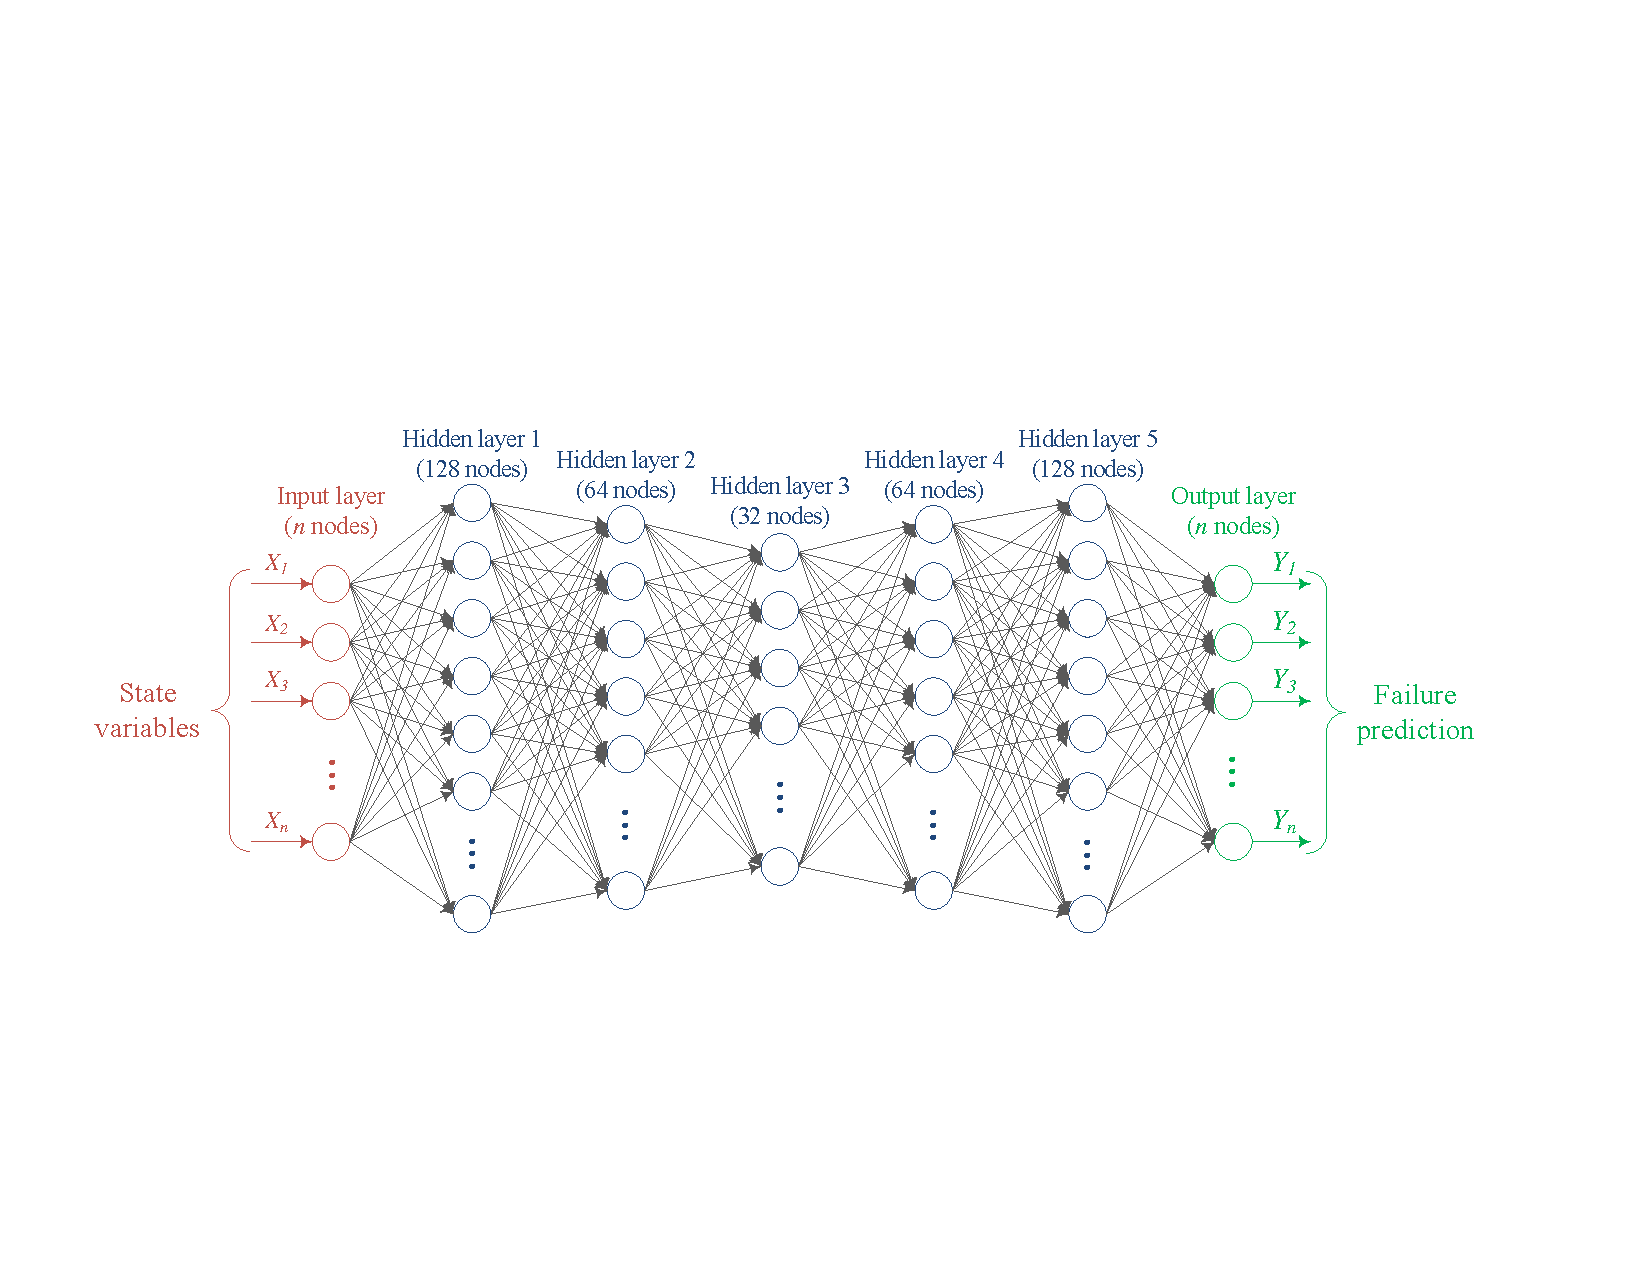
\includegraphics[width=\columnwidth]{nn_architecture}
\caption{Architecture of the multi-layer fully connected ANN used for failure prediction.}
\label{nn_architecture}
\end{figure}

%A \emph{decision function} $f(.)$ takes $\mathbf{Y}$ and returns binary failure predictions. In this work, the decision function is chosen to be a simple comparator with a predefined threshold $\eta$ as shown in Equation \eqref{eqn:decision_func}.
%
%\begin{equation}
%f(Y_i) =
%\left\{
%  \begin{array}{ll}
%    1, & \hbox{$Y_i > \eta$;} \\
%    0, & \hbox{otherwise.}
%  \end{array}
%\right. \quad , \quad 1 \leq i \leq n
%\label{eqn:decision_func}
%\end{equation}

In the nodes of the hidden layers, we have used the softplus activation function~\cite{DuB00}, which is a differentiable and smooth version of the well-known rectifier function, to introduce nonlinearity to the ANN. The optimizer used for updating weights of the ANN is Adam, as introduced in~\cite{KiB15}, and the loss function is found by calculating the cross entropy between the sigmoid of the failure predictions and that of the actual failures. In order to prevent overfitting during the training process, we utilized the $L_2$ regularization method, which penalizes the network for large weights by increasing the loss.

\hl{The choice of ANN architecture is generally based on heuristic rules. In this paper, the neural network is means to and end - demonstrating applicability of our method. Our choice of number and size of the hidden layers is based on previous studies on the performance of different ANNs in classification and time series prediction problems~\cite{YuS11}. The bottleneck hidden layer structure we used is known to create a compact representation of the information, and hence, acts as a nonlinear transformation and dimensionality reduction stage for the inputs. The number of hidden layers was further refined  through experimentation with available failure records and according to the quantitative performance metrics that we later discuss in Section \ref{sec:pred:metrics}. The number of nodes for each layer are chosen as powers of two to ensure computationally optimal matrix multiplications. Overall, the architecture presented here has shown excellent performance on the test cases investigated in Section \ref{sec:case_study}; however, depending on the type and size of the system under test, reconfiguration and adjustments may be necessary.}

The ANN is trained using a data set generated by simulating a number of failure cases or data from historical information of previous disruptions. In either case, each entry of the data set should include the state variables of the components at the time of the disruptive event (input to the ANN), linked with the list of components affected consequently (used as ground truth for optimization during training and verification). In Section \ref{sec:case_study:pred}, we demonstrate the application of this ANN and provide its performance in predicting failures for two smart grid examples.

Depending on the type of the system, preventive actions may be prioritized based on different parameters. Examples of prioritization parameters are the predicted failure probability of each component (provided by the neural network), importance of each component in providing essential services, and consequences of failure of each component on other components (e.g., weighted out-degree, as defined in Section \ref{sec:analysis:quan}) as well as on the operation of the system (e.g., in terms of loss of dependability~\cite{WoM20}).

\subsection{Evaluation of Predictive Performance}
\label{sec:pred:metrics}
In order to evaluate the effectiveness of the proposed ANN in predicting failures, we should use metrics that capture the predictive performance. To this end, we take advantage of the available metrics in the areas of information retrieval and classification, namely, accuracy, precision, recall, and $F_1$ score.

\emph{Accuracy} is a measure of correct classification, but has shortcomings in capturing the performance when the number of failed components is small compared to the total number of components, which is the case in our application. \emph{Precision} shows the ratio of successful failure detections to total detections. Precision also has a shortcoming in evaluating the performance when the ANN correctly predicts only a portion of the failed components, but fails to detect the remainder. \emph{Recall}, also known as sensitivity, is the ratio of the failed components detected by the ANN to the total number of failures. The shortcoming of recall is that its value is large if the ANN simply predicts that all of the components will fail. Therefore, no single metric is enough for evaluating the performance correctly. The \emph{$F_1$ score} has been introduced to solve this issue by combining precision and recall into a single metric by taking their harmonic mean. Equation \eqref{eqn:perf_measures} shows how these metrics are calculated.

\begin{eqnarray}
\text{Accuracy} &=& \frac{tp + tn}{tp + tn + fp + fn} \nonumber \\
\text{Precision} &=& \frac{tp}{tp + fp} \nonumber \\
\text{Recall} &=& \frac{tp}{tp + fn} \nonumber \\
\text{$F_1$ score} &=& 2 \times \frac{\text{Precision} \times \text{Recall}}{\text{Precision} + \text{Recall}}
\label{eqn:perf_measures}
\end{eqnarray}

In Equation \eqref{eqn:perf_measures}, $tp$, $tn$, $fp$, and $fn$ represent the numbers of true positives, true negatives, false positives, and false negatives, respectively.

\section{Case Study on Smart Grids}
\label{sec:case_study}
In this section, we demonstrate our proposed approach by applying it to two smart grids based on test systems well-studied in power engineering literature, namely, the IEEE 14-- and IEEE 57--bus test systems~\cite{PSTCA}. The IEEE 14--bus system has been included in the interest of brevity and clarity and the IEEE 57--bus system demonstrates the scalability of our method. These systems are depicted in \figurename~\ref{fig:ieee_bus_systems}.

\begin{figure}[H]
\centering
\subfloat[IEEE 14--bus smart grid]
{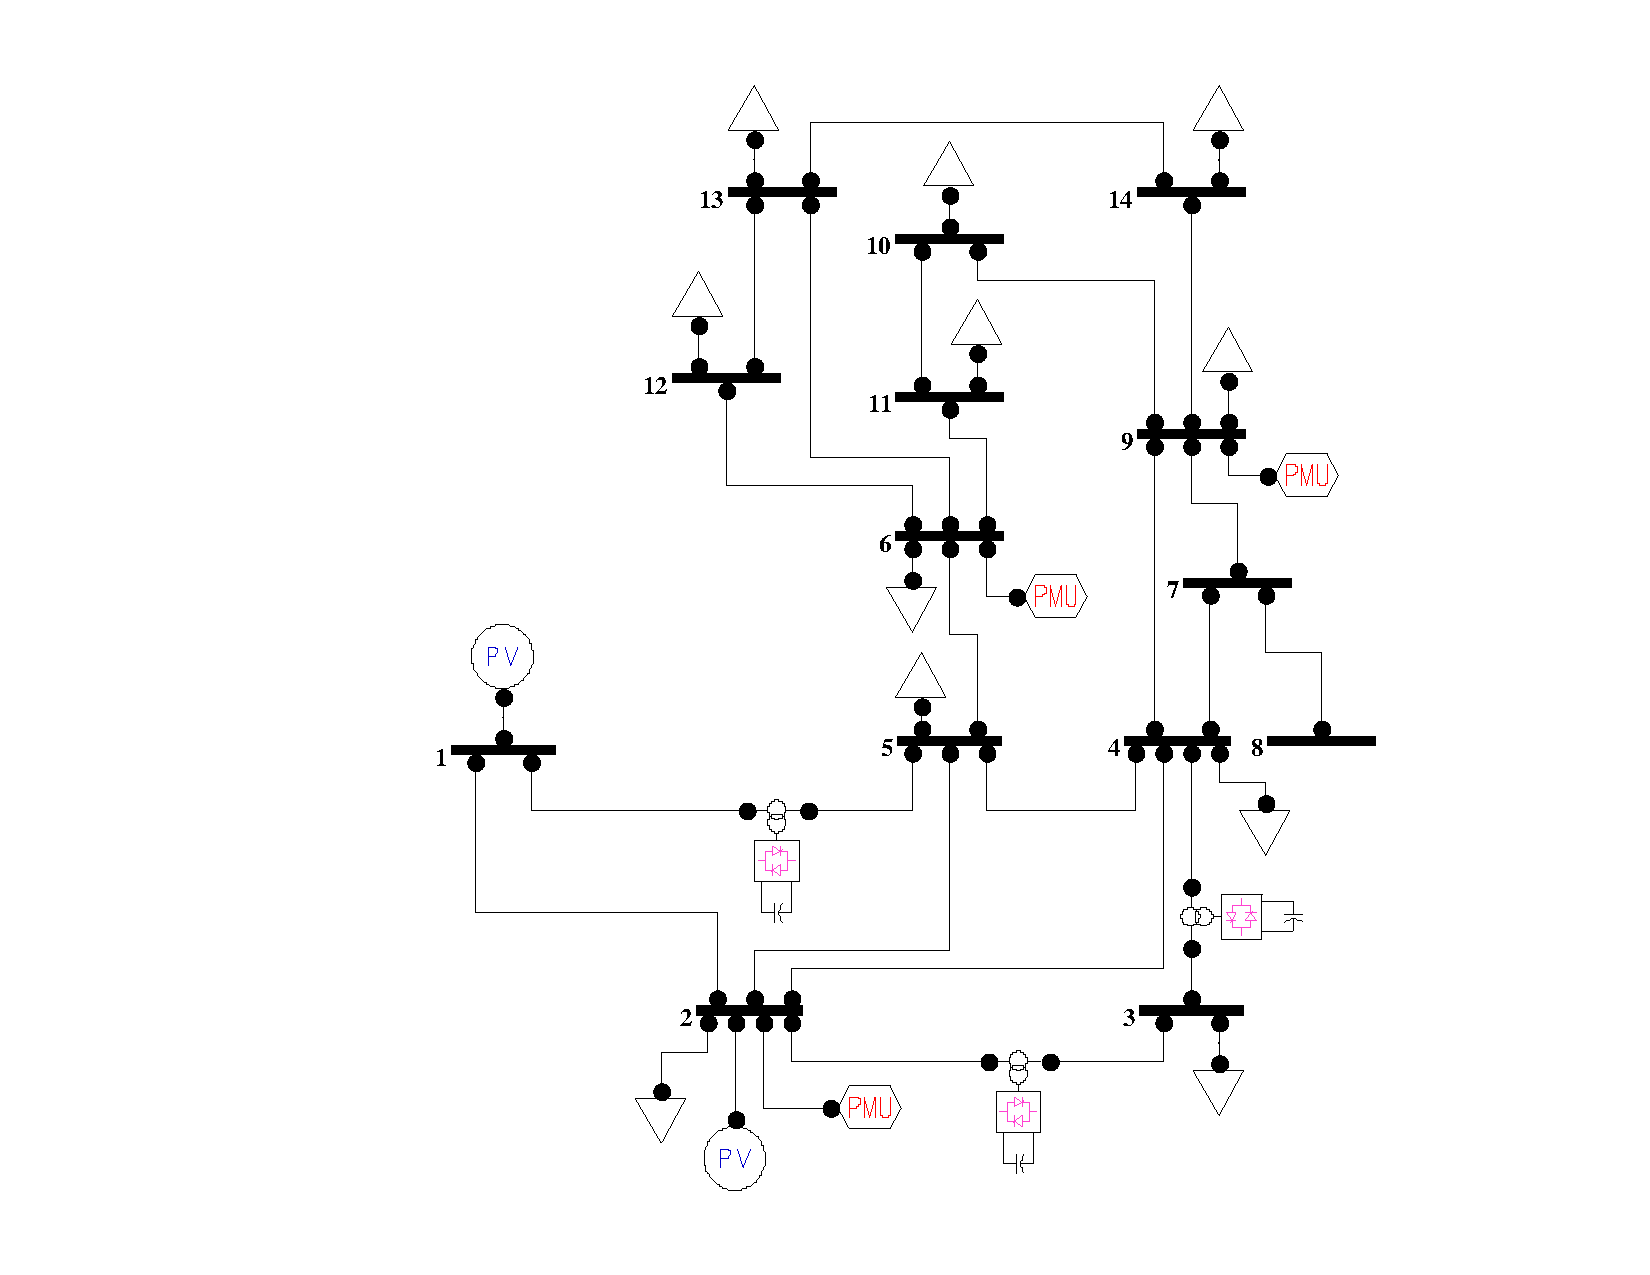
\includegraphics[width=0.45\columnwidth]{ieee14}
\label{fig:ieee14}}
~
\subfloat
{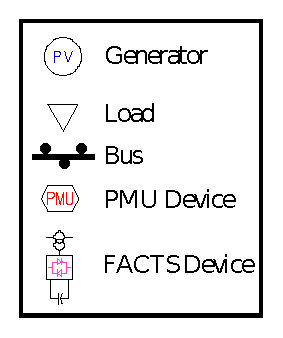
\includegraphics[width=0.20\columnwidth]{ieee_cases_legend}
\label{fig:ieee_legend}}

\setcounter{subfigure}{1}
\subfloat[IEEE 57--bus smart grid]
{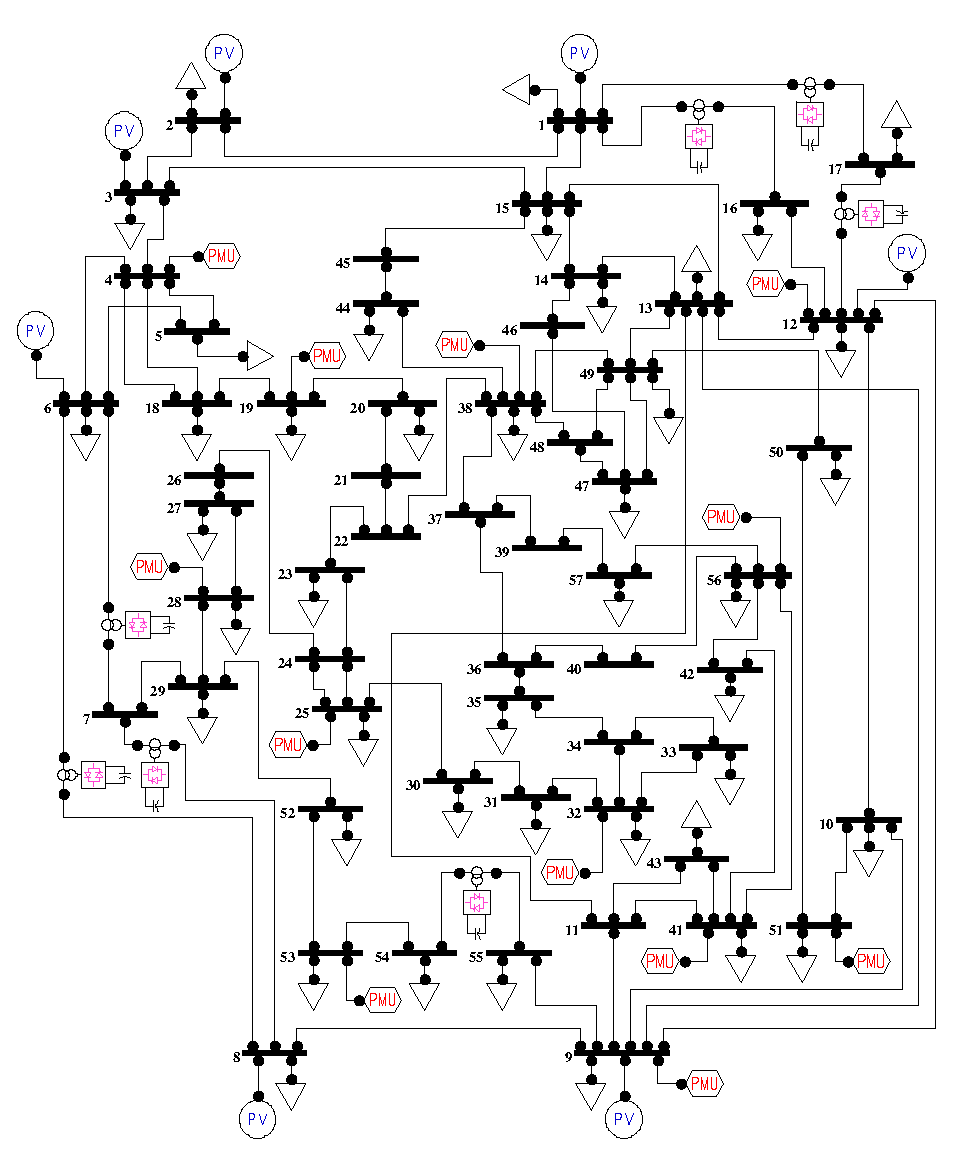
\includegraphics[width=0.60\columnwidth]{ieee57}
\label{fig:ieee57}}
\caption{Single line diagrams of IEEE smart grid test systems.}
\label{fig:ieee_bus_systems}
\end{figure}

The classic IEEE test systems do not utilize any advanced cyber technologies and are merely composed of generators, transmission lines, transformers, buses, and loads. Since our approach is intended to be applicable to cyber-physical systems, we supplemented the classic IEEE test systems with cyber infrastructure to create equivalent smart grid systems for demonstration purposes. The cyber infrastructure is comprised of phasor measurement units (PMU), which record and communicate GPS-synchronized dynamic power system data, flexible AC transmission system (FACTS) devices, which adjust the flow of power in the transmission lines, and a decision support algorithm that determines optimal settings for the FACTS devices based on data from the PMUs. We applied the methods presented in~\cite{AsK11} and~\cite{AcM07} to determine the locations of the PMUs and FACTS devices on each smart grid (shown in \figurename~\ref{fig:ieee_bus_systems}). We used a single-layer perceptron (not to be confused with the other ANN used for failure prediction introduced in Section \ref{sec:pred}) trained with $N-1$ contingencies as the decision support algorithm. For a more detailed explanation of the utilized cyber control scheme, readers are referred to our previous work~\cite{MaS14,MaS18}. In the remainder of this paper, we use the following notations for the aforementioned components:

\begin{itemize}
  \item $L_{i-j}$: A transmission line connecting bus $i$ to bus $j$
  \item $F_{i-j}$: A series FACTS device installed on line $L_{i-j}$
  \item $P_i$: A PMU installed at bus $i$
  %\item $CM_i$: A communication link between two cyber entities as shown on the test cases
  \item $DS$: The decision support algorithm
\end{itemize}

In addition to the intrinsic functional dependencies between components of smart grids, we assumed that the operation of PMU devices depends on the underlying power grid, i.e., a PMU device is disabled as soon as a voltage violation occurs at the bus on which it is installed. Voltage violation is defined to be outside of 0.9 to 1.1 per-unit range, according to the EN-50160 standard~\cite{EN50160}. Note that we consciously simplify this dependency (no backup power or fallback mechanism) as it allows us to better understand the consequences of the dependency of the cyber network on the physical system.

\subsection{Selection of Failure Cases}
\label{sec:case_study:selection}
Selecting failure cases and determining the minimum number of failure cases needed for obtaining all of the dependencies are of great importance in the presented method. In general, the larger the number of failure cases is, the more accurate the model becomes; however, exhaustive examination of failure cases is infeasible for large systems. The study presented in~\cite{QiS15} provides a method for selection of failure cases in analysis of power grids while a given accuracy is maintained. In this work, we analyzed the following scenarios:

\begin{itemize}
  \item One or two simultaneous transmission line outages,
  \item at most one failed FACTS device,
  \item at most one failed PMU, and
  %\item at most one failed communication channel, and
  \item failure of the decision support algorithm.
\end{itemize}

It is worth mentioning that upon availability of simulation environments capable of modeling the communication infrastructure with high resolution, considering the effects of respective impairments will improve the quality of the model. Unless a sophisticated model for channel impairments is utilized, inclusion of communication failures simply adds redundant failure cases and complicates representation of the results without actually capturing the behavior of data transport mechanisms. Therefore in this work, we have aggregated the failures of each communication link with those of the cyber component that receives the respective data. For example, a corrupted data package transmitted to a FACTS device is captured as a FACTS failure. Incorporating the manifestations of communication impairments guarantees that the model, despite the simplification, maintains all cyber-physical interdependencies. For instance, influence of a faulty PMU data on the operation of the decision support algorithm and corresponding FACTS device represents cyber-cyber dependencies.

Table~\ref{tab:failure_cases} lists the number of simulations carried out for each test case. The total number of simulations for each system is the product of the number of failure cases shown for each category of component. Note that in all of the failure cases at least one transmission line is tripped since it is observed that the system does not degrade otherwise, even in the presence of cyber faults; however, once one or more transmission lines has tripped, impairment of cyber components can exacerbate the situation and lead to further degradation.

\begin{table}[!t]
\caption{Number of simulated failure cases.}
\label{tab:failure_cases}
\footnotesize
\centering
\renewcommand{\arraystretch}{1.3}
\begin{tabular}{m{0.22\columnwidth}|c|c}
  & IEEE--14 & IEEE--57 \\ \hline
  transmission lines & $\sum\limits_{k=1}^2\binom{20}{k} = 210$ & $\sum\limits_{k=1}^2\binom{80}{k} = 3,240$ \\
  FACTS devices & $\sum\limits_{k=0}^1\binom{3}{k} = 4$ & $\sum\limits_{k=0}^1\binom{7}{k} = 8$ \\
  PMU devices & $\sum\limits_{k=0}^1\binom{3}{k} = 4$ & $\sum\limits_{k=0}^1\binom{12}{k} = 13$ \\
  %communication links & $\sum\limits_{k=0}^1\binom{6}{k} = 7$ & $\sum\limits_{k=0}^1\binom{19}{k} = 20$ \\
  decision support & $\sum\limits_{k=0}^1\binom{1}{k} = 2$ & $\sum\limits_{k=0}^1\binom{1}{k} = 2$ \\ \hline
  \textbf{total number of simulated cases} & \textbf{6,720} & \textbf{673,920}
\end{tabular}
\end{table}

In this study, failure cases were selected based on the failure rate of components. Transmission lines were selected because they have a relatively high rate of failure and are a major source of power outages~\cite{SoW13}. Additionally, we selected FACTS and PMU devices and the decision support as representative cyber components because their failure can impact the state of the physical components. Including other components of the system can enhance the model and improve the accuracy of results.

\subsection{Simulations}
\label{sec:case_study:sim}
For the electric delivery system, there are a number of commercial and non-commercial computer simulation tools available. The PowerWorld Simulator~\cite{PwrWrld} is a popular commercial tool for analysis of high voltage power systems. It supports common protection and control devices, provides an interactive environment and intuitive GUI, and is able to solve power flow equations for very large systems; however, PowerWorld does not provide the transparency needed for analysis of the sequence of failures. Several other commercial software packages, such as DIgSILENT~\cite{DIg}, have the same shortcoming. Among the non-commercial packages, MATPOWER~\cite{MATPWR} and PSAT~\cite{Mi05} are two MATLAB-based toolboxes for Windows machines. MATPOWER can solve load flow and optimal power flow problems in a command line interface. PSAT has a graphical interface and supports basic monitoring and protection devices and power regulators in addition to the capabilities of MATPOWER. In this work, we used PSAT for simulation of the two IEEE bus systems. For the purpose of our simulations, we enhanced PSAT in order to achieve the high resolution required for analysis of smart grids~\cite{MaS14,MaS18}. These enhancements include incorporating wide-area measurement capabilities by PMU devices, providing a platform for implementing a decision support algorithm, and integrating the power systems with communication technologies used in smart grid applications. This modified version of PSAT is interfaced with a MATLAB wrapper that acts as an adapter between libraries and orchestrates subroutine calls.

The simulation environment is used to determine power flows and voltages in the system during the failure cases. For each failure case, specific faults are injected to predetermined components of the system by disabling FACTS devices, PMU devices, and decision support as well as tripping transmission lines. At each time step, PSAT performs power flow analysis and determines active power flow on each line and voltage at each bus. Active power flow of the lines are compared to their capacity, and if any line is overloaded, it is considered failed and the topology is updated accordingly. Since the cyber-physical dependencies are incorporated in the data models and enforced by the simulation environment, the propagation of the injected faults takes place automatically. For example, when the decision support platform receives a faulty data from a malfunctioning PMU, it is likely to send incorrect commands to respective FACTS devices. The FACTS devices will in turn apply wrong compensations and decrease power transfer capability of the system. The resulting load imbalance can overload and trip transmission lines and cause further cyber and/or physical failures. The simulation continues this automatic propagation of faults until no further failures are detected.

\subsection{Interdependencies of IEEE Bus Systems}
\label{sec:case_study:interdep}
In this section, we present interdependencies of IEEE--14 and IEEE--57 smart grids identified using both correlation and causation analyses. Correlation analysis requires state variable for each component to be defined. Equation~\eqref{eqn:state_variables} shows definition of state variables for each category of components in smart grids.

\begin{eqnarray}
X_{L_{i-j}}(t) &=& |\text{\footnotesize Active power flow of $L_{i-j}$ in p.u. at time $t$}| \nonumber \\
X_{F_{i-j}}(t) &=& \left\{
                     \begin{array}{ll}
                       1, & \hbox{\text{\footnotesize $F_{i-j}$ is operational at time $t$};} \\
                       0, & \hbox{\text{\footnotesize otherwise}.}
                     \end{array}
                   \right. \nonumber \\
X_{P_{i}}(t) &=& \left\{
                     \begin{array}{ll}
                       1, & \hbox{\text{\footnotesize $P_{i}$ is operational at time $t$};} \\
                       0, & \hbox{\text{\footnotesize otherwise}.}
                     \end{array}
                   \right. \nonumber \\
X_{DS}(t) &=& \dfrac{\text{\footnotesize Number of observable buses and lines}}{\text{\footnotesize Total number of buses and lines}}
\label{eqn:state_variables}
\end{eqnarray}

In Equation~\eqref{eqn:state_variables}, $X_{L_{i-j}}(t) \in \mathbb{R}^+$, $X_{F_{i-j}}(t)\in \{0, 1\}$, $X_{P_{i}}(t) \in \{0, 1\}$, and $X_{DS}(t) \in [0, 1]$. Note that $X_{DS}(t)$ is the portion of the power system that is observable to the decision support and is used as a measure since it well captures its operation and data dependency on PMU devices. \figurename~\ref{fig:state_variables} shows how these state variables can capture the operation of a smart grid during a failure sequence. In \figurename~\ref{fig:state_variables}, state variables of components of IEEE--14 smart grid during a selected failure sequence are plotted on a single horizontal axis. Note that the state variables are shown for components that experience degradation only. Each row presents the state variable of a component. The rows are ordered according to the propagation of the faults, i.e., the two topmost rows correspond to the components whose failure initiates the failure case ($L_{1-5}$ and $P_2$); the third and fourth rows represent state variable of the components that fail consequently ($L_{1-2}$ and $F_{1-5}$); and so forth.

\begin{figure}
\centering
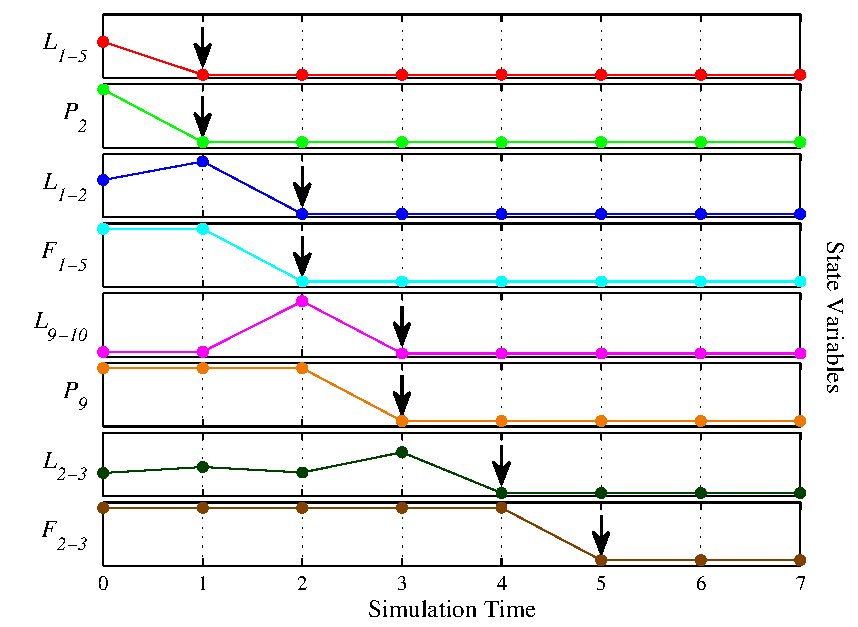
\includegraphics[width=0.65\columnwidth]{state_variables}
\caption{State variables of selected components of IEEE--14 during a failure sequence. Arrows indicate the points at which components are considered failed.}
\label{fig:state_variables}
\end{figure}

According to \figurename~\ref{fig:state_variables}, the correlation among the state variables is expected to be maximal for those which degrade with one time step difference. Table~\ref{tab:cor_state_variables} shows values of $PCC$ and $RDC$ for pairs of components that degrade with one time step difference as shown in \figurename~\ref{fig:state_variables}. In calculation of $RDC$ values, sample size and number of random features are set to 0.1 and 1, respectively.

\begin{table}
\centering
\caption{Correlation coefficients between state variables of component pairs for those experience degradation with one time step difference in the failure case shown in \figurename~\ref{fig:state_variables}.}
\label{tab:cor_state_variables}
\begin{tabular}{ll|cc}
\multicolumn{2}{c|}{State variables} & $PCC$ & $RDC$ \\ \hline
$X_{L_{1-5}}$  & $X_{L_{1-2}}$       & 1.00  & 1.00  \\
$X_{L_{1-5}}$  & $X_{F_{1-5}}$       & 1.00  & 1.00  \\
$X_{P_{2}}$    & $X_{L_{1-2}}$       & 1.00  & 1.00  \\
$X_{P_{2}}$    & $X_{F_{1-5}}$       & 1.00  & 1.00  \\
$X_{L_{1-2}}$  & $X_{L_{9-10}}$      & 0.85  & 1.00  \\
$X_{L_{1-2}}$  & $X_{P_{9}}$         & 0.98  & 1.00  \\
$X_{F_{1-5}}$  & $X_{L_{9-10}}$      & 0.71  & 1.00  \\
$X_{F_{1-5}}$  & $X_{P_{9}}$         & 1.00  & 1.00  \\
$X_{L_{9-10}}$ & $X_{L_{2-3}}$       & 0.79  & 0.99  \\
$X_{P_{9}}$    & $X_{L_{2-3}}$       & 0.95  & 0.99  \\
$X_{L_{2-3}}$  & $X_{F_{2-3}}$       & 0.94  & 0.99  \\[2pt] \hline
\multicolumn{2}{m{0.26\columnwidth}|}{Maximum among all other pairs} & 0.68 & 0.83
\end{tabular}
\end{table}

% NJ - Mention an example of the nonlinear interdep. captured by RDC; perhaps F1-5 and L9-10
Both correlation coefficients exhibit relatively large values for the component pairs that are expected to have dependence; however, $RDC$ values of dependent components better stand out according to Table~\ref{tab:cor_state_variables}. This is mainly due to the fact that $RDC$ captures nonlinear as well as linear correlations, unlike $PCC$, which only captures linear relationships and results in underestimating dependency between component pairs that are non-linearly correlated. Hereinafter, we utilize and present $RDC$ values only, due to its superiority in capturing interdependence.

For each failure case, $RDC$ values are calculated for all pairs of state variables. For estimating $d_{ij}$ the mean value of $RDC_{X_i X_j}$ is calculated over all failure cases. Likewise, the process explained in Section \ref{sec:analysis:iden:caus} is applied on the results of simulations to find the $d_{ij}$ values using causation analysis. For each of the methods, we found $d_{ij}$ values and constructed the $\mathbf{D}$ matrix.

$\mathbf{D}$ matrices are visually represented as weighted directed graphs in \figurename~\ref{fig:ieee14_graph} and \figurename~\ref{fig:ieee57_graph} for IEEE--14 and IEEE--57 smart grid systems. Each edge represents a direct dependency and its width is proportional to the extent of the dependence ($d_{ij}$). Note that edges with weights less than 0.05 are not shown in the figures for ease of illustration. The top five links with largest weights are shown in red. It can be seen that dependency links with large weights are captured by both correlation and causation methods. It is also seen that the correlation-based method identifies a larger number of direct dependencies, as causation is typically a relationship that exists only in a small fraction of correlated events (also seen in \figurename~\ref{wij_hist}).

%TODO - Use magenta instead of orange (nodes)
\begin{figure}[H]
\centering
\subfloat[Correlation (RDC)]
{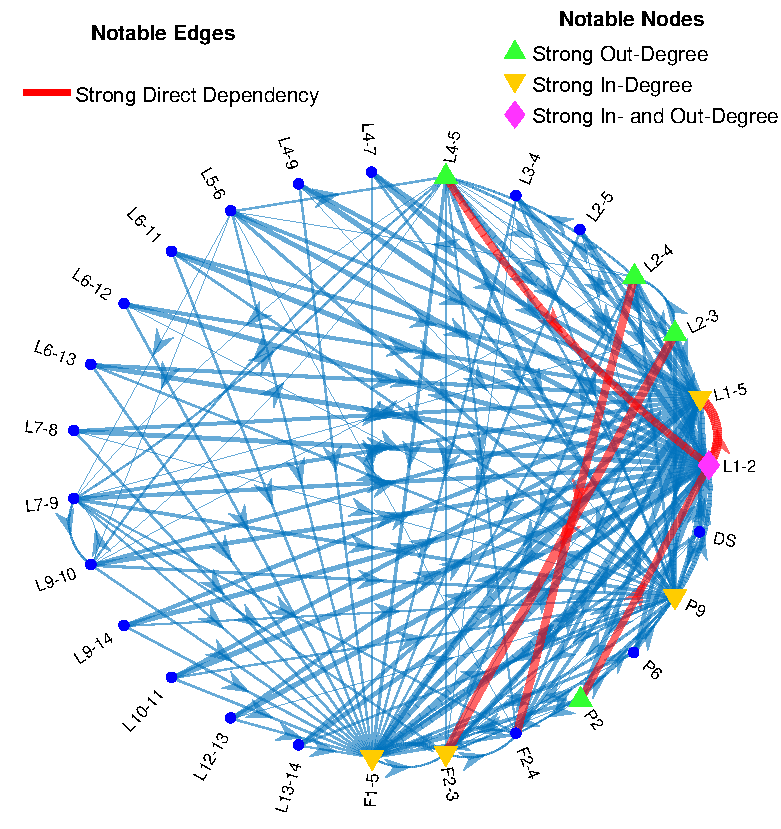
\includegraphics[width=0.48\columnwidth]{ieee14_graph_rdc}
\label{fig:ieee14_graph_rdc}}
~
\subfloat[Causation]
{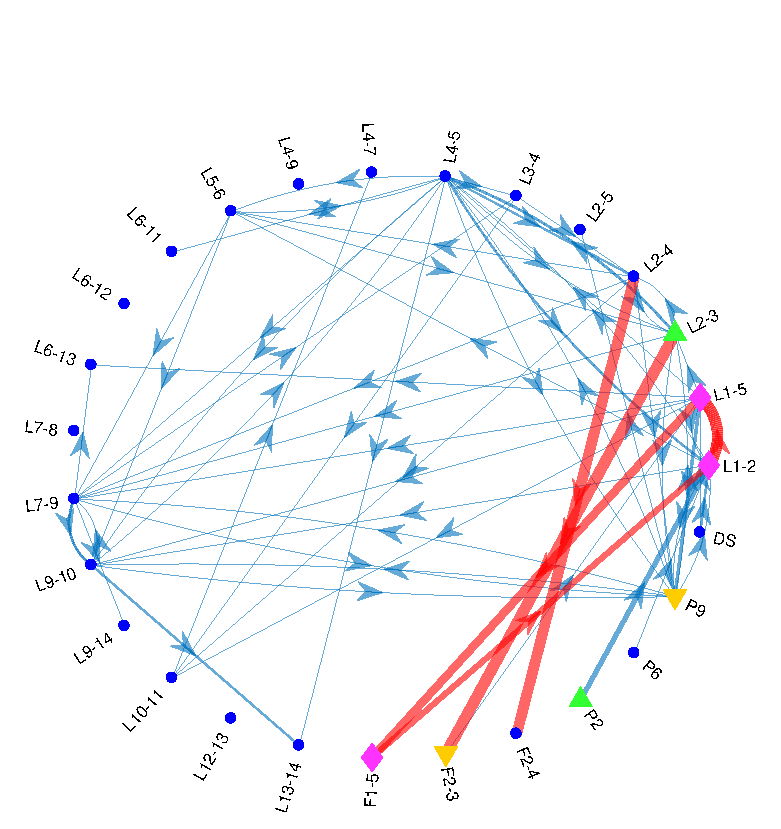
\includegraphics[width=0.48\columnwidth]{ieee14_graph_causation}
\label{fig:ieee14_graph_causation}}
\caption{Graph representation of $\mathbf{D}$ matrix for IEEE--14 smart grid identified using correlation \protect\subref{fig:ieee14_graph_rdc} and causation \protect\subref{fig:ieee14_graph_causation} analyses. Notable dependency links are shown in red.}
\label{fig:ieee14_graph}
\end{figure}

%TODO - Use magenta instead of orange (nodes)
\begin{figure}[H]
\centering
\subfloat[Correlation (RDC)]
{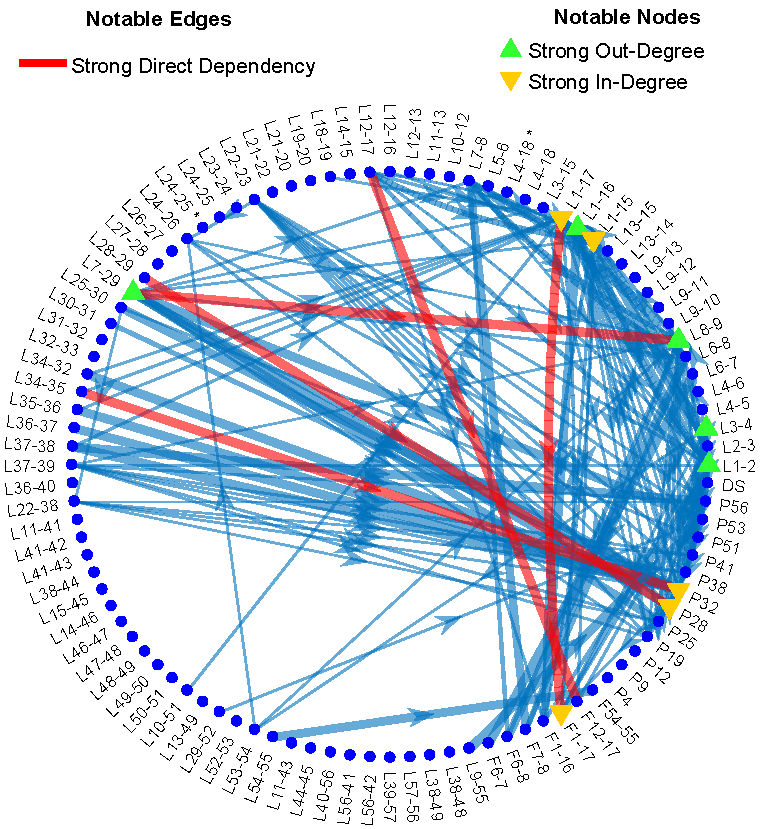
\includegraphics[width=0.48\columnwidth]{ieee57_graph_rdc}
\label{fig:ieee57_graph_rdc}}
~
\subfloat[Causation]
{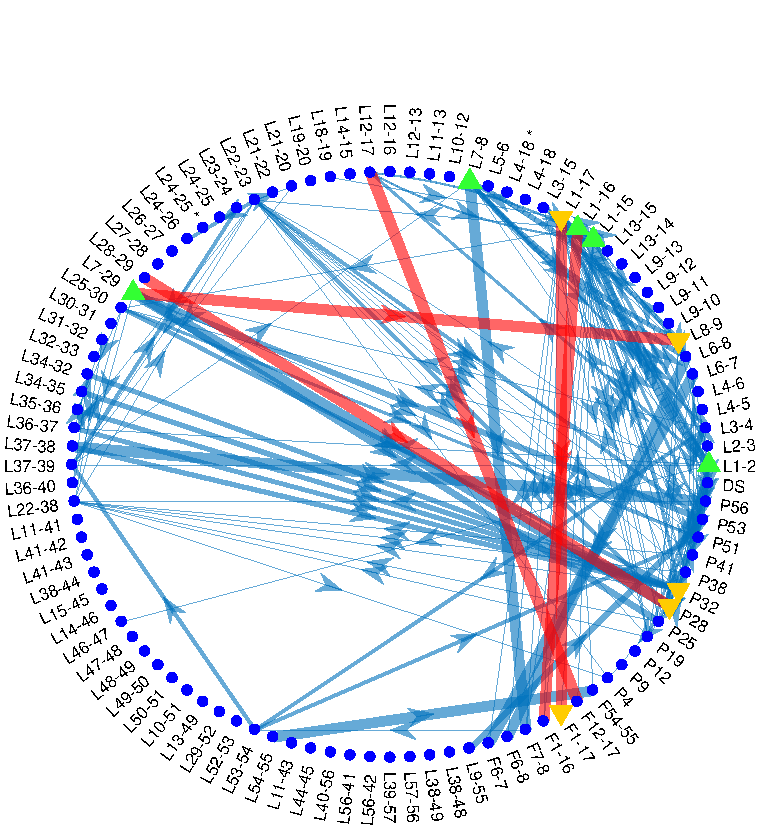
\includegraphics[width=0.48\columnwidth]{ieee57_graph_causation}
\label{fig:ieee57_graph_causation}}
\caption{Graph representation of $\mathbf{D}$ matrix for IEEE--57 smart grid identified using correlation \protect\subref{fig:ieee57_graph_rdc} and causation \protect\subref{fig:ieee57_graph_causation} analyses. Notable dependency links are shown in red.}
\label{fig:ieee57_graph}
\end{figure}

To verify correctness of the causation links identified, further analytical study is required. For the sake of brevity, we present our analysis on only the top five causation links shown in \figurename~\ref{fig:ieee14_graph_causation} for IEEE-14. The most fragile section of the IEEE-14 system is the combination of $L_{1-2}$ and $L_{1-5}$. In normal operation, the load on $L_{1-5}$ is very small and the majority of the power is transmitted to the rest of the grid through $L_{1-2}$. In research studies on standard power test systems the capacity of each transmission line is usually assumed to be 120\% or 125\% of its power flow in normal operation. With this assumption, the capacity of $L_{1-5}$ is significantly lower than that of $L_{1-2}$, and hence, upon tripping of $L_{1-2}$, the additional power flow that will have to be transmitted through $L_{1-5}$ causes an overload. This confirms the causation link of $L_{1-2} - L_{1-5}$. In all cases of $L_{2-3} - F_{2-3}$, $L_{2-4} - F_{2-4}$, and $L_{1-5} - F_{1-5}$ a tripped transmission line causes its FACTS device to fail. These causation link are also valid as the FACTS devices are rendered inoperative upon outage of the respective transmission lines. Finally, the causation link of $F_{1-5} - L_{1-2}$ is valid as the only means of controlling the balance between $L_{1-2}$ and $L_{1-5}$ is through $F_{1-5}$, and hence, failure of $F_{1-5}$ creates and imbalance that leads to an overload on $L_{1-2}$.

%TODO - Show some of the notable total influence links with nonlocal property on the IEEE cases
By applying interdependency quantification methods presented in Section \ref{sec:analysis:quan}, we computed the $\mathbf{T}$ matrix based on  direct dependencies identified using both correlation and causation analyses. From the values of $t_{ij}$ we can see links that are of great importance. As an example, in the IEEE--14 smart grid case, the total influence from the decision support to $L_{1-5}$ is among the largest values while the corresponding direct link has a small weight of 0.05. The pair of $P_{32}$ and $F_{1-17}$ in the IEEE--57 smart grid is another example of a similar situation. This characteristic is justified by existence of several multi-step strong dependency links that connect pairs of components together and can give rise to further breakdown of components that are not in the geographical, logical, physical, or cyber reach of the initially impaired component~\cite{RiP01}. This nonlocal property of the fault propagation has been observed in a number of real-world blackouts~\cite{BeA04,A14Rp}.

In \figurename~\ref{fig:ieee14_graph} and \figurename~\ref{fig:ieee57_graph}, the top five components (nodes) with highest in-degree ($\nu$) and out-degree ($\tau$) values are specified by distinguishable markers. This analysis identifies the cyber and physical elements that have the highest priority for further inspection and fortification if dependability is to be improved. Among the identified components are the bridge lines, which are responsible for transmitting the majority of the power from the generating buses to the load buses, as well as PMU and FACTS devices that are installed at critical locations of the power grid. Identifying these components using analytical methods can be very difficult or even impossible for large systems.

%To improve the robustness of a system with a dependency graph that shows components with high in-degree and/or out-degree:
%in-degree: increasing the capacity of existing components to prevent overload, replace with more robust components, utilizing redundant components~\cite{AvL04]
%out-degree: employing a diverse selection of components. Diversity involves the use of spatially, temporally, and functionally different alternatives~\cite{StH10}.

In order to compare the extent of dependency among the cyber and physical subsystems, $\gamma_{s_1-s_2}$ is calculated and shown in \figurename~\ref{fig:gamma}.

\begin{figure}
\centering
\subfloat[IEEE--14 smart grid]
{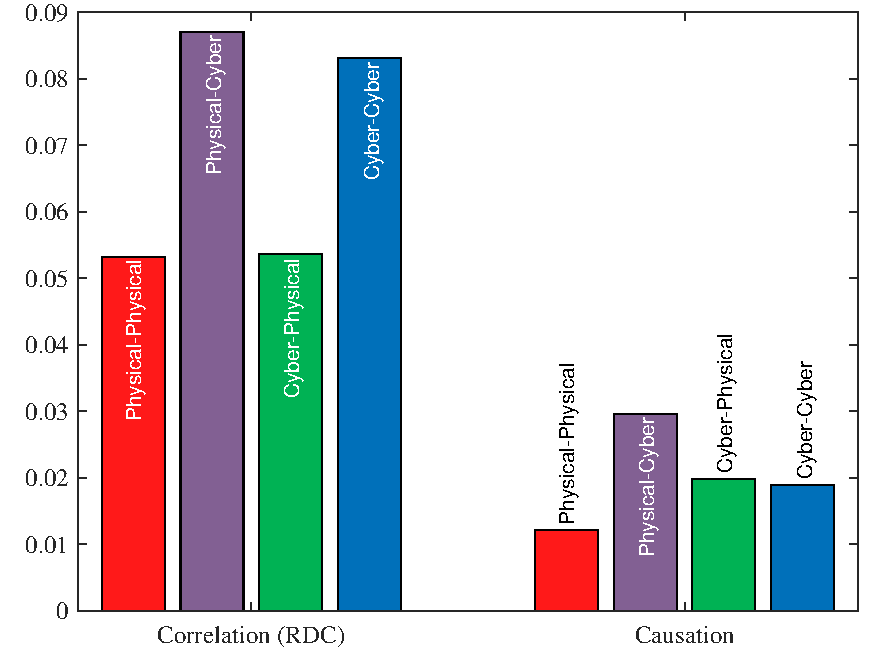
\includegraphics[width=0.48\columnwidth]{ieee14_gamma}
\label{fig:ieee14_gamma}}
~
\subfloat[IEEE--57 smart grid]
{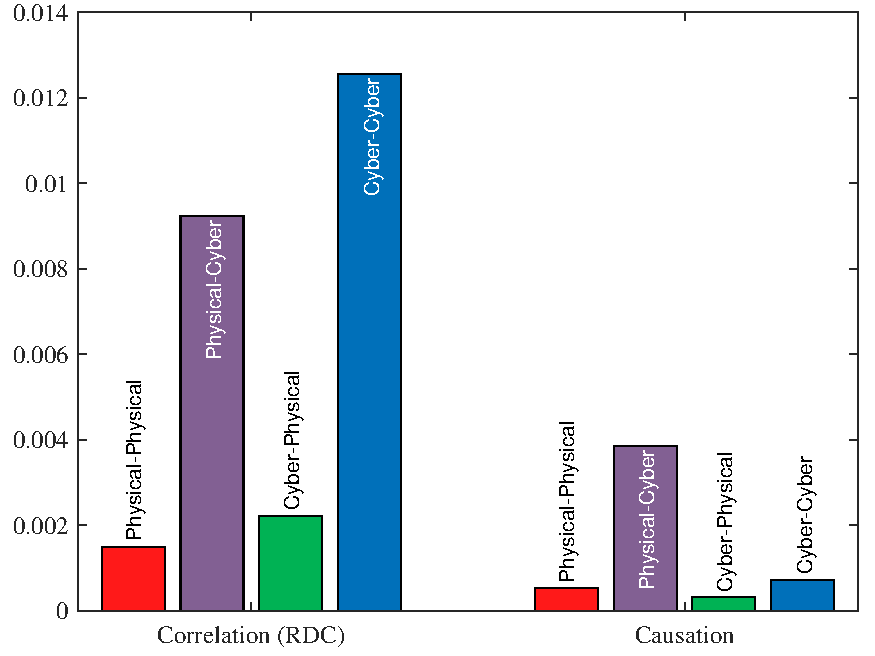
\includegraphics[width=0.48\columnwidth]{ieee57_gamma}
\label{fig:ieee57_gamma}}
\caption{Comparison of dependency among subsystems ($\gamma_{s_1-s_2}$) using correlation and causation analyses.}
\label{fig:gamma}
\end{figure}

It can be seen that the most significant dependencies are from the physical subsystem to the cyber subsystem (physical-cyber) and within the cyber subsystem (cyber-cyber). Dependency of cyber components on the physical components are typically in binary form (e.g., if power is not available the sensor shuts off) which justifies the large value of corresponding $\gamma_{s_1-s_2}$ value. The large value of cyber-cyber dependency is mainly due to the nature of the common topologies of the cyber infrastructure, in which each component is connected to multiple other components for transmission and reception of information.

Comparing the respective $\gamma_{s_1-s_2}$ values obtained from the correlation and causation analyses, we can infer that the causation relationships among the components are less frequent and of smaller extent, which can also be observed in the graphs provided in \figurename~\ref{fig:ieee14_graph} and \figurename~\ref{fig:ieee57_graph}; however, the orders of $\gamma_{s_1-s_2}$ values within each group are similar to each other.

\subsection{Prediction of Failures}
\label{sec:case_study:pred}
For training the ANN, we need to convert the failure data into a data set composed of several input/output elements. \figurename~\ref{fig:failure_seq} shows an example of a failure sequence for a hypothetical system with eight components. In this failure case, the system initially has faults in components 2 and 6. The faulty state is propagated to other components and affects component 1, then components 4 and 8, and finally component 5. We then transform this failure case into four entries of the data set used for training the ANN, as shown in the right of \figurename~\ref{fig:failure_seq}. Each entry of the data set has two fields: i) an array of the state variables at a time instance and ii) a list of components that will degrade at the next time step.

\begin{figure}
\centering
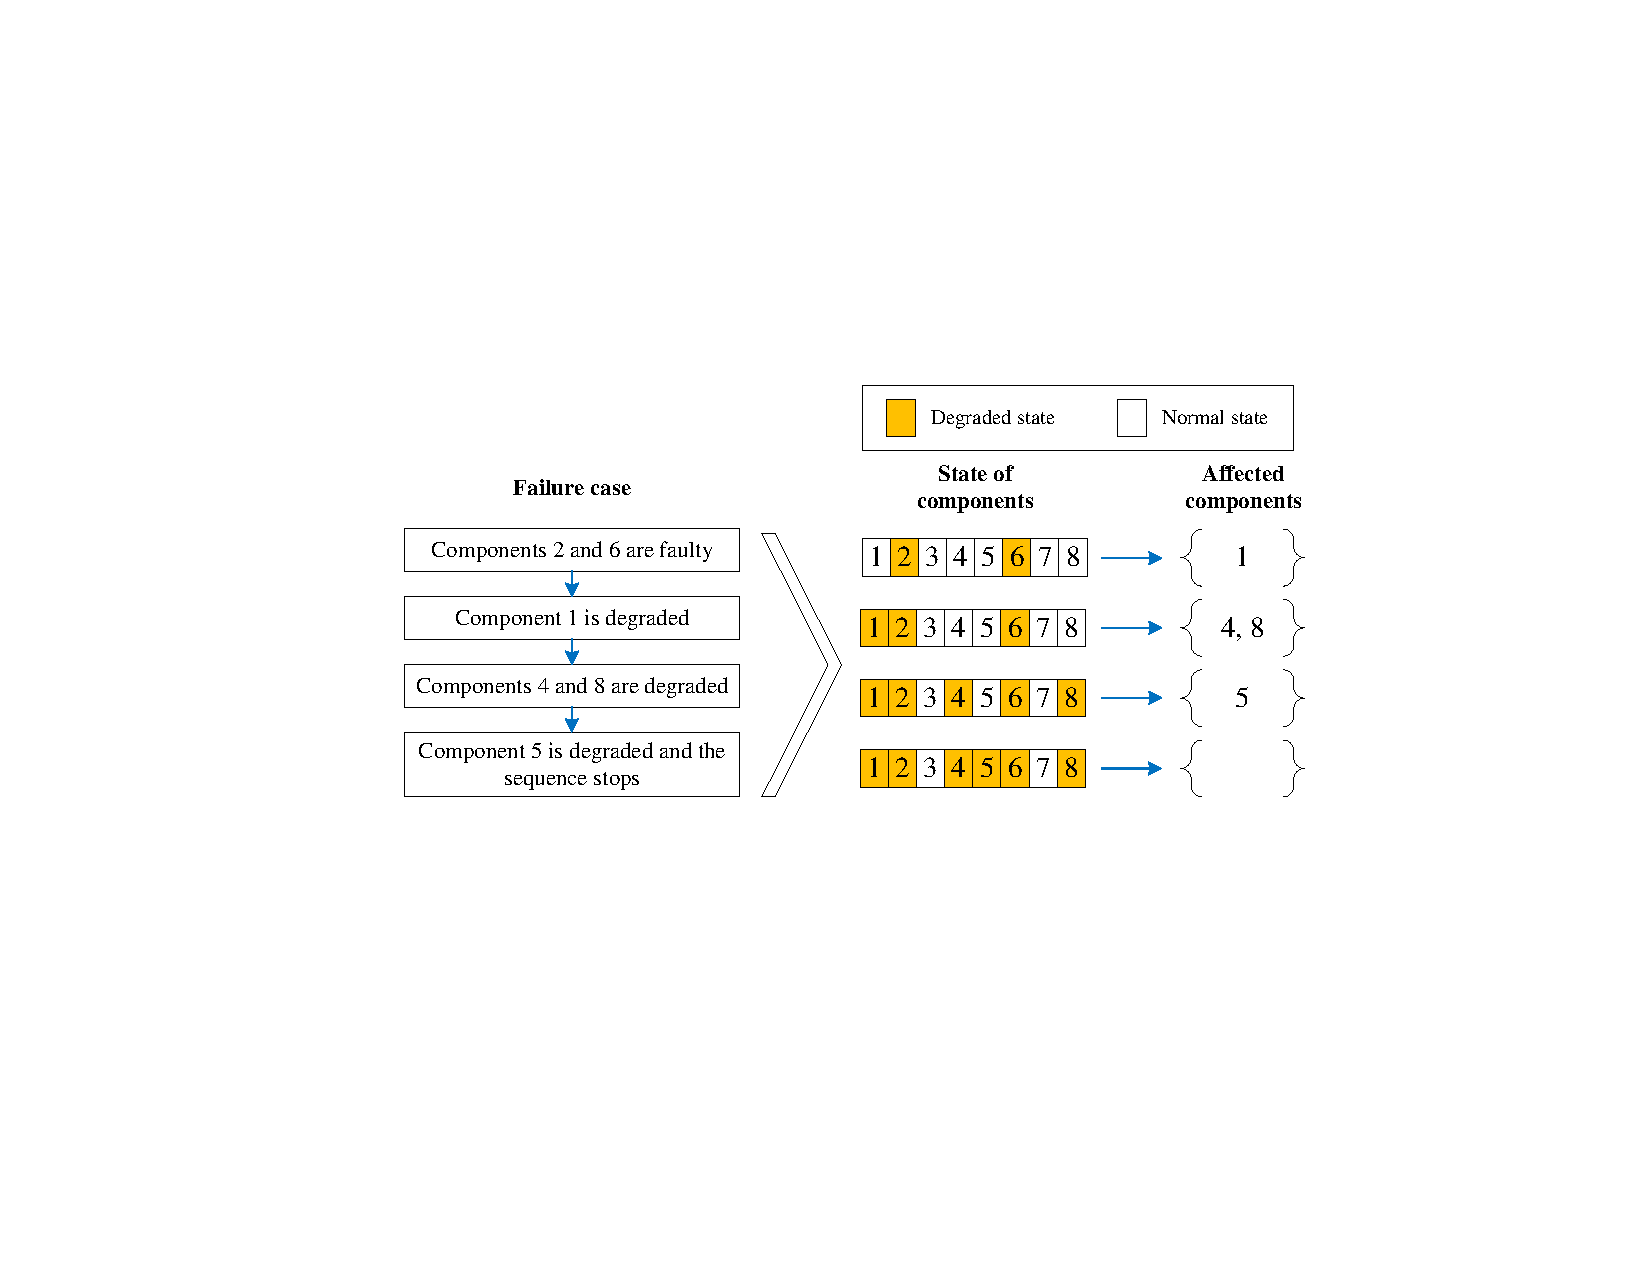
\includegraphics[width=0.75\columnwidth]{failure_seq}
\caption{Transformation of a failure sequence into four entries of the data set used for training the ANN.}
\label{fig:failure_seq}
\end{figure}

The failure cases simulated for IEEE--14 and IEEE--57 smart grids resulted in data sets with several entries. Since the failure data for real-world large-scale CPSs is limited, we will investigate the possibility of training the ANN with a small subset of the available data sets and inspect its predictive capability. We randomly selected a subset of the available data and then divided them into training, validation, and test data sets using random selection. The training data set is used for adjusting the weights of the ANN shown in Section \ref{sec:pred} by back propagation, while the validation data set is employed as a recurrent feedback loop to minimize prediction error during the training cycles. This separation of training and validation data sets is done to prevent overfitting of the neural network. An overfitted model is one that corresponds very closely to the training data set, and hence, may fail to make accurate predictions on future observations. Upon completion of the training, the test data set is used for measuring the predictive performance of the ANN.

We also simulated a number of randomly selected more complex failure cases for each smart grid system and evaluated the performance of the ANN on predicting failures on those cases. The difference between the ``simple'' and the ``complex'' test data is that the latter is composed of failure cases with three to five concurrent transmission line failures, while the former is selected from the failure cases explained in Table \ref{tab:failure_cases}, where at most two transmission lines are tripped concurrently. Table \ref{tab:nn_data} shows the number of entries of the failure data used for the ANN.

\begin{table}
\caption{Size of the failure data sets used for the ANN.}
\label{tab:nn_data}
\centering
\renewcommand{\arraystretch}{1.1}
\begin{tabular}{ll|l|l}
\multicolumn{2}{c|}{Data set}                              & IEEE--14 & IEEE--57  \\ \hline
\multicolumn{2}{l|}{Total failure data available}         & 17,968   & 1,181,871 \\
\multicolumn{2}{l|}{Simple failure data used for the ANN} & 10,000   & 20,000    \\
 & Training data (80\%)                                   & 8,000    & 16,000    \\
 & Validation data (10\%)                                 & 1,000    & 2,000     \\
 & Test data (10\%)                                       & 1,000    & 2,000     \\
\multicolumn{2}{l|}{Complex test data}                    & 1,000    & 1,000     \\
\end{tabular}
\end{table}

Predictions on the failure cases from the complex data sets are expected to be harder for the ANN as they are not of the same type of the input data by which the ANN is trained. Performance measures of the ANN on simple and complex test data sets are shown in Table \ref{tab:nn_perf}. It is worth mentioning that the failure prediction process, from inputting the system state to the ANN until receiving the output in the form of component indices that are about to fail, takes less than one millisecond on an Intel Xeon E5-2623 3.00 GHz machine. For implementation of the ANN, we used the TensorFlow package 1.2.0~\cite{AbA15} in Python 3.6.0.

\begin{table}
\caption{Predictive performance measures of the ANN.}
\label{tab:nn_perf}
\centering
\renewcommand{\arraystretch}{1.1}
\begin{tabular}{rl|ccc}
System                    & Test Data & Precision & Recall  & $F_1$ score \\ \hline % & Accuracy
\multirow{2}{*}{IEEE--14} & Simple    & 99.25\%   & 98.21\% & 98.46\%     \\        % & 99.46\%
                          & Complex   & 90.63\%   & 83.65\% & 85.54\%     \\ \hline % & 98.18\%
\multirow{2}{*}{IEEE--57} & Simple    & 99.38\%   & 98.66\% & 98.87\%     \\        % & 99.94\%
                          & Complex   & 84.83\%   & 71.55\% & 75.29\%               % & 99.16\%
\end{tabular}
\end{table}

As seen in Table \ref{tab:nn_perf}, the ANN has an excellent performance on the simple data sets, both for IEEE--14 and IEEE--57 smart grids. Although the ANN does not perform as well on the complex data sets, its performance is still acceptable. The fact that the ANN can predict imminent failures with a high accuracy is mainly in virtue of the interdependence among the components and existence of recurred failure sequences. Identification of such sequences of failure that frequently occur is also useful in fortification of the system~\cite{WoM20}.

As mentioned earlier, we have performed the case study on a larger test system based on the IEEE--57 in order to evaluate the scalability of our approach. From Table \ref{tab:nn_perf}, we can see that the ANN has a similar performance for IEEE--14 and IEEE-57 systems. Considering the fact that IEEE--14 is composed of 27 components (20 transmission lines, 3 FACTS devices, 3 PMU devices, and 1 decision support platform) while IEEE--57 has a total of 100 components (80 transmission lines, 7 FACTS devices, 12 PMU devices, and 1 decision support platform), the $100/27 \approx 3.7 \times$ increase in the size of the system only requires a $2 \times$ increase in the size of the training failure data set from 8,000 to 16,000 (Table \ref{tab:nn_data}). This verifies the scalability of our prediction approach and its applicability to large-scale systems.

Thus far, we have seen that the ANN has a good performance in detecting the components that are about to fail, both with high accuracy and high speed. Another equally important feature of a prediction tool is that it maintains its performance when it is trained with a relatively small data set. In order to investigate whether the proposed approach has this feature and to find the minimum number of required entries in the training data set, we have performed the training process with subsets of the available data set and measured the predictive performance of the resulting ANN on a fixed test data set. \figurename~\ref{fig:nn_training_size} shows how the performance measures of the ANN in predicting failures of the IEEE--14 and IEEE--57 smart grids are affected by varying the size of the training data set.

\begin{figure}[!h]
\centering
\subfloat[IEEE--14 smart grid]
{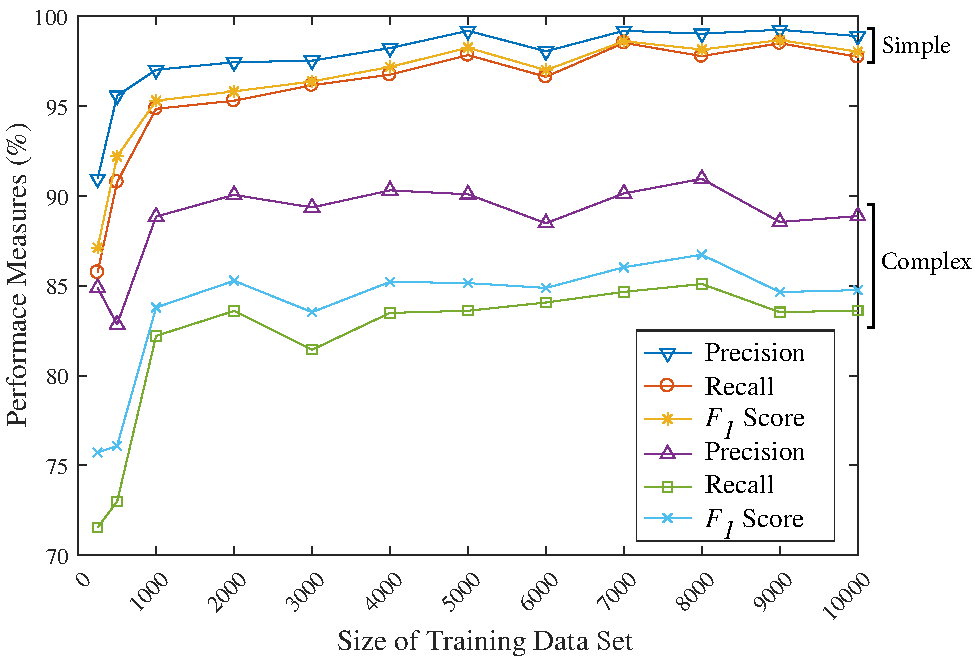
\includegraphics[width=0.65\columnwidth]{ieee14_tr_sz}
\label{fig:ieee14_tr_sz}}

\subfloat[IEEE--57 smart grid]
{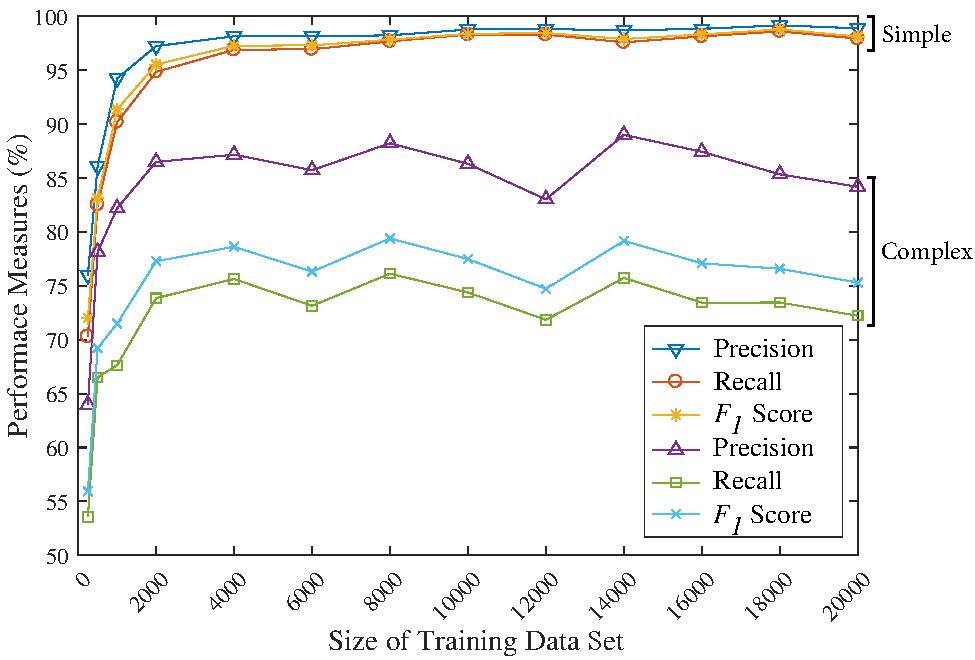
\includegraphics[width=0.65\columnwidth]{ieee57_tr_sz}
\label{fig:ieee57_tr_sz}}
\caption{The effect of the size of training data set on predictive performance of the ANN.}
\label{fig:nn_training_size}
\end{figure}

As expected, it is seen in \figurename~\ref{fig:nn_training_size} that the performance of the ANN degrades as we decrease the size of the training data set. Note that due to the randomness in selection of the training data, the performance curves are not monotonically increasing. According to \figurename~\ref{fig:nn_training_size}, increasing the size of the training data set to more than 1000 for IEEE--14 smart grid and 2000 for IEEE--57 smart grid does not have a significant effect on the predictive performance of the ANN. Since the performance of the proposed ANN is not contingent on having large training data sets it can be trained using data available in the reports of the past power outages for developing a failure prediction tool for smart grids.

\section{Conclusions}
\label{sec:conc}
\sout{The research presented in this paper investigates the use of correlation and causation metrics for detection and quantification of the extent of dependency links among the components of a CPS. We provided the interdependency metrics, which seek to capture the effect of the multi-step dependencies as well as the immediate dependency links. These interdependency metrics revealed a number of dependency links among the components which previously were indiscernible. Such component pairs are not in the geographical, logical, physical, or cyber reach of each other, nevertheless are strongly dependent. This nonlocal property of the fault propagation has been observed in the past and was shown on the test cases in this paper.

We also proposed a neural network approach for prediction of imminent component failures. Partly due to the high level of interdependence among the components of the analyzed systems, the neural network shows excellent predictive performance. This setup could detect the forthcoming failures with a high $F_1$ score of 98\% on IEEE-14 and IEEE-57 smart grids. As shown by several studies, such high level of interdependency and recurred failure sequences exist in most of the critical infrastructures, and hence, this failure prediction approach can be efficiently applied to other domains. In the future of this research, we will take into account the effect of communication failures and consider more advanced ANN architectures in order to incorporate temporal features of the failures as well.}

\hl{In this paper, we illuminate interdependencies among the components of a CPS using correlation metrics, and a heuristic causation analysis method, respectively. We propose quantitative metrics for the extent of dependency among components, aiming to reflect both immediate and gradual failure propagation. We illustrate use of this information in detecting  nonlocal fault propagation, which occurs among  components without  geographical, logical, physical, or cyber proximity. This in turn enables the prediction of imminent failures, which we demonstrated using a neural network approach. For smart grids based on the IEEE-14 and IEEE-57 test systems, we were able to predict forthcoming failures with an $F_1$ score of 98\%. We plan to extend this research by considering the effect of communication failures and investigating the use of  more advanced machine learning methods for failure prediction.}% and evaluate effectiveness of the proposed prediction technique in facilitating failure prevention

\section*{Acknowledgments}
We gratefully acknowledge support from the US Departments of Education and Transportation for funding this project.

\bibliography{bib_db}

\ifappendix
  \newpage
  \appendix
  \section{Largest Dependency Links ($d_{ij}$)}
  \begin{table}[H]
\centering
\caption{Notable dependencies among components of IEEE-14 smart grid.}
\label{tab:d_ieee14}
\footnotesize
\setlength{\tabcolsep}{2pt}
\begin{tabular}{l@{ - }lc|l@{ - }lc|l@{ - }lc}
\multicolumn{3}{c}{\textbf{PCC}} & \multicolumn{3}{c}{\textbf{RDC}} & \multicolumn{3}{c}{\textbf{Causation}} \\
\multicolumn{2}{c}{Components} & $d_{ij}$ & \multicolumn{2}{c}{Components} & $d_{ij}$ & \multicolumn{2}{c}{Components} & $d_{ij}$ \\ \hline
$L_{1-2}$ & $L_{1-5}$ & 0.73 & $L_{1-2}$ & $L_{1-5}$ & 0.83 & $L_{1-2}$ & $L_{1-5}$  & 0.83 \\
$L_{2-3}$ & $F_{2-3}$ & 0.60 & $L_{2-3}$ & $F_{2-3}$ & 0.79 & $L_{2-3}$ & $F_{2-3}$  & 0.81 \\
$L_{2-4}$ & $F_{2-4}$ & 0.52 & $L_{2-4}$ & $F_{2-4}$ & 0.72 & $L_{2-4}$ & $F_{2-4}$  & 0.77 \\
$P_{2}$   & $L_{1-2}$ & 0.49 & $L_{4-5}$ & $L_{1-2}$ & 0.61 & $L_{1-5}$ & $F_{1-5}$  & 0.56 \\
$F_{1-5}$ & $L_{1-2}$ & 0.48 & $P_{2}$   & $L_{1-2}$ & 0.60 & $F_{1-5}$ & $L_{1-2}$  & 0.39 \\
$L_{4-5}$ & $L_{1-2}$ & 0.45 & $F_{1-5}$ & $L_{1-2}$ & 0.57 & $P_{2}$   & $L_{1-2}$  & 0.32 \\
$L_{1-5}$ & $F_{1-5}$ & 0.43 & $L_{1-5}$ & $F_{1-5}$ & 0.56 & $L_{1-5}$ & $P_{9}$    & 0.20 \\
$F_{1-5}$ & $L_{1-5}$ & 0.35 & $F_{1-5}$ & $L_{1-5}$ & 0.52 & $L_{2-3}$ & $L_{4-5}$  & 0.13 \\
$L_{2-3}$ & $L_{1-5}$ & 0.34 & $L_{1-5}$ & $L_{1-2}$ & 0.46 & $DS$      & $L_{1-2}$  & 0.12 \\
$L_{4-9}$ & $L_{1-2}$ & 0.33 & $L_{2-3}$ & $L_{1-5}$ & 0.46 & $L_{7-9}$ & $L_{9-10}$ & 0.12
\end{tabular}
\end{table}

\begin{table}[H]
\centering
\caption{Notable dependencies among components of IEEE-57 smart grid.}
\label{tab:d_ieee57}
\footnotesize
\setlength{\tabcolsep}{2pt}
\begin{tabular}{l@{ - }lc|l@{ - }lc|l@{ - }lc}
\multicolumn{3}{c}{\textbf{PCC}} & \multicolumn{3}{c}{\textbf{RDC}} & \multicolumn{3}{c}{\textbf{Causation}} \\
\multicolumn{2}{c}{Components} & $d_{ij}$ & \multicolumn{2}{c}{Components} & $d_{ij}$ & \multicolumn{2}{c}{Components} & $d_{ij}$ \\ \hline
$L_{1-17}$  & $F_{1-17}$  & 0.76 & $L_{7-29}$  & $L_{8-9}$   & 0.96 & $L_{12-17}$ & $F_{12-17}$ & 0.95 \\
$L_{7-29}$  & $L_{8-9}$   & 0.73 & $L_{12-17}$ & $F_{12-17}$ & 0.94 & $L_{1-17}$  & $F_{1-17}$  & 0.94 \\
$L_{12-17}$ & $F_{12-17}$ & 0.72 & $L_{1-17}$  & $F_{1-17}$  & 0.93 & $L_{28-29}$ & $P_{28}$    & 0.92 \\
$L_{2-3}$   & $L_{1-15}$  & 0.69 & $L_{28-29}$ & $P_{28}$    & 0.92 & $L_{7-29}$  & $L_{8-9}$   & 0.92 \\
$F_{1-16}$  & $F_{1-16}$  & 0.68 & $L_{34-35}$ & $P_{32}$    & 0.92 & $L_{1-16}$  & $F_{1-16}$  & 0.91 \\
$L_{7-8}$   & $F_{7-8}$   & 0.67 & $L_{9-55}$  & $P_{53}$    & 0.92 & $L_{37-38}$ & $P_{56}$    & 0.91 \\
$L_{34-35}$ & $P_{32}$    & 0.65 & $L_{37-38}$ & $P_{32}$    & 0.92 & $L_{7-8}$   & $F_{7-8}$   & 0.91 \\
$L_{28-29}$ & $P_{28}$    & 0.65 & $L_{37-38}$ & $P_{56}$    & 0.92 & $L_{6-7}$   & $F_{6-7}$   & 0.90 \\
$L_{9-55}$  & $P_{53}$    & 0.65 & $L_{34-32}$ & $P_{32}$    & 0.91 & $L_{54-55}$ & $F_{54-55}$ & 0.88 \\
$L_{37-38}$ & $P_{32}$    & 0.65 & $L_{35-36}$ & $P_{32}$    & 0.91 & $L_{7-29}$  & $P_{28}$    & 0.87
\end{tabular}
\end{table} 
  \section{Largest Multi-step Dependency Links ($t_{ij}$)}
  \begin{table}[H]
\centering
\caption{Notable multi-step dependency links among components of IEEE-14 smart grid; dependency links that are relatively large in $\mathbf{T}$, but small in $\mathbf{D}$.}
\label{tab:t_ieee14}
\footnotesize
\begin{tabular}{l@{ - }l|l@{ - }l|l@{ - }l}
\multicolumn{2}{c}{\textbf{PCC}} & \multicolumn{2}{c}{\textbf{RDC}} & \multicolumn{2}{c}{\textbf{Causation}} \\
\multicolumn{2}{c|}{Components} & \multicolumn{2}{c|}{Components} & \multicolumn{2}{c}{Components} \\ \hline
$L_{2-3}$ & $L_{1-2}$ & $L_{2-3}$ & $L_{1-2}$ & $L_{1-2}$ & $F_{1-5}$ \\
$L_{4-5}$ & $L_{1-5}$ & $L_{2-3}$ & $L_{1-5}$ & $F_{1-5}$ & $L_{1-5}$ \\
$L_{2-3}$ & $L_{1-5}$ & $L_{4-5}$ & $L_{1-5}$ & $P_{2}$ & $L_{1-5}$ \\
$L_{2-4}$ & $L_{1-5}$ & $L_{2-4}$ & $L_{1-5}$ & $L_{1-5}$ & $L_{1-2}$ \\
$L_{2-3}$ & $F_{1-5}$ & $L_{2-3}$ & $F_{1-5}$ & $L_{1-2}$ & $P_{9}$ \\
$L_{2-3}$ & $L_{1-2}$ & $L_{2-4}$ & $L_{1-2}$ & $P_{2}$ & $F_{1-5}$ \\
$P_{2}$ & $L_{1-5}$ & $L_{2-4}$ & $F_{1-5}$ & $DS$ & $L_{1-5}$ \\
$L_{2-4}$ & $L_{1-2}$ & $L_{4-5}$ & $F_{1-5}$ & $F_{1-5}$ & $P_{9}$ \\
$L_{2-4}$ & $F_{1-5}$ & $L_{5-6}$ & $L_{1-5}$ & $L_{4-5}$ & $L_{1-5}$ \\
$L_{5-6}$ & $L_{1-5}$ & $L_{7-9}$ & $L_{1-5}$ & $DS$ & $F_{1-5}$
\end{tabular}
\end{table}

\begin{table}[H]
\centering
\caption{Notable multi-step dependency links among components of IEEE-57 smart grid; dependency links that are relatively large in $\mathbf{T}$, but small in $\mathbf{D}$.}
\label{tab:t_ieee57}
\footnotesize
\begin{tabular}{l@{ - }l|l@{ - }l|l@{ - }l}
\multicolumn{2}{c}{\textbf{PCC}} & \multicolumn{2}{c}{\textbf{RDC}} & \multicolumn{2}{c}{\textbf{Causation}} \\
\multicolumn{2}{c|}{Components} & \multicolumn{2}{c|}{Components} & \multicolumn{2}{c}{Components} \\ \hline
$L_{7-29}$ & $L_{1-15}$ & $L_{7-29}$ & $L_{1-15}$ & $L_{7-29}$ & $L_{7-8}$ \\
$L_{7-29}$ & $L_{1-2}$ & $L_{7-29}$ & $L_{1-2}$ & $L_{7-8}$ & $F_{6-8}$ \\
$L_{7-29}$ & $F_{7-8}$ & $L_{7-29}$ & $F_{7-8}$ & $L_{8-9}$ & $F_{7-8}$ \\
$L_{7-29}$ & $P_{32}$ & $L_{1-16}$ & $P_{32}$ & $L_{1-16}$ & $L_{1-2}$ \\
$L_{7-29}$ & $F_{1-17}$ & $L_{7-29}$ & $F_{1-17}$ & $L_{7-29}$ & $L_{6-8}$ \\
$L_{7-29}$ & $L_{1-17}$ & $L_{7-29}$ & $L_{1-17}$ & $L_{1-15}$ & $F_{1-17}$ \\
$L_{1-16}$ & $P_{32}$ & $L_{7-29}$ & $P_{32}$ & $L_{8-9}$ & $F_{6-8}$ \\
$L_{7-29}$ & $L_{7-8}$ & $L_{1-2}$ & $P_{32}$ & $L_{1-2}$ & $F_{1-17}$ \\
$L_{1-15}$ & $P_{32}$ & $L_{1-15}$ & $P_{32}$ & $P_{32}$ & $F_{1-17}$ \\
$L_{8-9}$ & $L_{1-15}$ & $L_{1-16}$ & $F_{1-17}$ & $L_{1-2}$ & $F_{1-16}$
\end{tabular}
\end{table} 
  \section{Largest Out-degree Values ($\tau_i$)}
  \begin{table}[H]
\centering
\caption{Weighted out-degree of components of the IEEE-14 smart grid.}
\label{tab:tau_ieee14}
\footnotesize
\begin{tabular}{cc|cc|cc}
\multicolumn{2}{c}{\textbf{PCC}} & \multicolumn{2}{c}{\textbf{RDC}} & \multicolumn{2}{c}{\textbf{Causation}} \\
Component & $\tau$ & Components & $\tau$ & Component & $\tau$ \\ \hline
$L_{2-3}$ & 0.239 & $L_{2-3}$ & 0.244 & $L_{1-2}$ & 0.206 \\
$L_{4-5}$ & 0.219 & $L_{4-5}$ & 0.234 & $L_{1-5}$ & 0.187 \\
$L_{2-4}$ & 0.215 & $L_{2-4}$ & 0.220 & $L_{4-5}$ & 0.152 \\
$L_{1-2}$ & 0.205 & $L_{1-2}$ & 0.206 & $F_{1-5}$ & 0.143 \\
$P_{9}$ & 0.196 & $L_{7-9}$ & 0.200 & $L_{2-3}$ & 0.128 \\
$L_{1-5}$ & 0.193 & $P_{2}$ & 0.199 & $P_{2}$ & 0.127 \\
$F_{1-5}$ & 0.188 & $L_{5-6}$ & 0.197 & $L_{2-4}$ & 0.113 \\
$P_{2}$ & 0.187 & $L_{1-5}$ & 0.196 & $P_{9}$ & 0.093 \\
$F_{2-3}$ & 0.185 & $F_{1-5}$ & 0.194 & $DS$ & 0.091 \\
$L_{5-6}$ & 0.178 & $P_{9}$ & 0.191 & $L_{7-9}$ & 0.071
\end{tabular}
\end{table}

\begin{table}[H]
\centering
\caption{Weighted out-degree of components of the IEEE-57 smart grid.}
\label{tab:tau_ieee57}
\footnotesize
\begin{tabular}{cc|cc|cc}
\multicolumn{2}{c}{\textbf{PCC}} & \multicolumn{2}{c}{\textbf{RDC}} & \multicolumn{2}{c}{\textbf{Causation}} \\
Component & $\tau$ & Components & $\tau$ & Component & $\tau$ \\ \hline
$L_{7-29}$ & 0.073 & $L_{7-29}$ & 0.072 & $L_{1-2}$ & 0.047 \\
$L_{8-9}$ & 0.069 & $L_{1-16}$ & 0.067 & $L_{7-29}$ & 0.038 \\
$L_{1-2}$ & 0.063 & $L_{1-2}$ & 0.067 & $L_{1-15}$ & 0.033 \\
$L_{1-16}$ & 0.063 & $L_{8-9}$ & 0.067 & $L_{1-16}$ & 0.031 \\
$L_{1-15}$ & 0.062 & $L_{1-15}$ & 0.063 & $L_{7-8}$ & 0.028 \\
$L_{7-8}$ & 0.055 & $L_{3-4}$ & 0.060 & $L_{22-23}$ & 0.025 \\
$P_{25}$ & 0.053 & $L_{22-23}$ & 0.060 & $L_{8-9}$ & 0.024 \\
$L_{12-17}$ & 0.052 & $L_{37-39}$ & 0.058 & $L_{1-17}$ & 0.018 \\
$P_{19}$ & 0.051 & $L_{7-8}$ & 0.056 & $L_{37-38}$ & 0.018 \\
$P_{28}$ & 0.050 & $L_{12-17}$ & 0.054 & $L_{6-8}$ & 0.016
\end{tabular}
\end{table} 
  \section{Largest In-degree Values ($\nu_j$)}
  \begin{table}[H]
\centering
\caption{Weighted in-degree of components of the IEEE-14 smart grid.}
\label{tab:nu_ieee14}
\footnotesize
\begin{tabular}{cc|cc|cc}
\multicolumn{2}{c}{\textbf{PCC}} & \multicolumn{2}{c}{\textbf{RDC}} & \multicolumn{2}{c}{\textbf{Causation}} \\
Component & $\nu$ & Components & $\nu$ & Component & $\nu$ \\ \hline
$L_{1-2}$ & 0.591 & $L_{1-5}$ & 0.604 & $L_{1-5}$ & 0.181 \\
$L_{1-5}$ & 0.575 & $L_{1-2}$ & 0.594 & $L_{1-2}$ & 0.1168 \\
$F_{1-5}$ & 0.497 & $F_{1-5}$ & 0.495 & $F_{1-5}$ & 0.151 \\
$P_{9}$ & 0.421 & $P_{9}$ & 0.427 & $P_{9}$ & 0.148 \\
$F_{2-3}$ & 0.318 & $F_{2-3}$ & 0.322 & $L_{4-5}$ & 0.118 \\
$F_{2-4}$ & 0.269 & $L_{4-5}$ & 0.285 & $L_{9-10}$ & 0.103 \\
$L_{4-5}$ & 0.263 & $F_{2-4}$ & 0.280 & $F_{2-3}$ & 0.101 \\
$L_{2-3}$ & 0.219 & $L_{9-10}$ & 0.237 & $L_{7-9}$ & 0.093 \\
$L_{9-10}$ & 0.187 & $L_{2-3}$ & 0.210 & $F_{2-4}$ & 0.088 \\
$L_{7-9}$ & 0.175 & $L_{7-9}$ & 0.208 & $L_{2-3}$ & 0.080
\end{tabular}
\end{table}

\begin{table}[H]
\centering
\caption{Weighted in-degree of components of the IEEE-57 smart grid.}
\label{tab:nu_ieee57}
\footnotesize
\begin{tabular}{cc|cc|cc}
\multicolumn{2}{c}{\textbf{PCC}} & \multicolumn{2}{c}{\textbf{RDC}} & \multicolumn{2}{c}{\textbf{Causation}} \\
Component & $\nu$ & Components & $\nu$ & Component & $\nu$ \\ \hline
$F_{1-17}$ & 0.130 & $L_{1-17}$ & 0.132 & $P_{32}$ & 0.045 \\
$L_{1-17}$ & 0.130 & $F_{1-17}$ & 0.128 & $L_{1-17}$ & 0.043 \\
$P_{32}$ & 0.116 & $P_{32}$ & 0.126 & $F_{1-17}$ & 0.031 \\
$L_{1-15}$ & 0.101 & $L_{1-15}$ & 0.109 & $L_{1-15}$ & 0.028 \\
$L_{1-2}$ & 0.086 & $L_{1-2}$ & 0.099 & $P_{28}$ & 0.027 \\
$P_{28}$ & 0.083 & $P_{25}$ & 0.092 & $P_{53}$ & 0.023 \\
$P_{25}$ & 0.081 & $P_{28}$ & 0.092 & $L_{8-9}$ & 0.022 \\
$P_{53}$ & 0.081 & $P_{53}$ & 0.089 & $P_{25}$ & 0.020 \\
$F_{1-16}$ & 0.077 & $F_{1-16}$ & 0.084 & $L_{7-8}$ & 0.019 \\
$F_{7-8}$ & 0.077 & $P_{56}$ & 0.084 & $P_{56}$ & 0.019
\end{tabular}
\end{table} 
\fi

\end{document}
